\documentclass[
    corpo=11pt,
    twoside,
]{toptesi}

%%%%%%%%%%%%%%%%%%%%%%%%%%%%%%%%%%%%%%%%%%%%%%%%%%%%%%%%%%%%%%%

\pdfpagewidth\paperwidth    % per assicurarsi che nel pdf
\pdfpageheight\paperheight  % sia riempita tutta la pagina

%%%%%%%%%%%%%%%%%%%%%%%%%%%%%%%%%%%%%%%%%%%%%%%%%%%%%%%%%%%%%%%

% LIBRERIE
\usepackage[classica]{topfront}     % frontespizio
\usepackage[utf8]{inputenc}         % utf8
\usepackage[italian]{babel}
\usepackage[T1]{fontenc}
\usepackage{lmodern}
%\usepackage{textcomp}               % provide many text symbols
%\usepackage{booktabs}
\usepackage{graphicx, wrapfig}
\usepackage[a-1b]{pdfx}
\usepackage{minted}                 % coding language
\usepackage{xurl}
\usepackage{epigraph}
\usepackage{amsthm}
\usepackage[babel]{csquotes}
\usepackage[backend=biber,bibencoding=ascii,sorting=none]{biblatex}

%%%%%%%%%%%%%%%%%%%%%%%%%%%%%%%%%%%%%%%%%%%%%%%%%%%%%%%%%%%%%%%

% CONFIGURAZIONE LINK E RIFERIMENTI
\hypersetup{%
    pdfpagemode={UseOutlines},
    bookmarksopen,
    pdfstartview={FitH},
    colorlinks,
    linkcolor={black}, %COLORE RIFERIMENTI INDICE
    citecolor={blue}, %COLORE CITAZIONI
    urlcolor={blue}, %COLORE URL
}

%%%%%%%%%%%%%%%%%%%%%%%%%%%%%%%%%%%%%%%%%%%%%%%%%%%%%%%%%%%%%%%

% CAPITOLI DA INCLUDERE
\includeonly{%
  chapters/stateofart,%
  chapters/systemdesign,%
}

%%%%%%%%%%%%%%%%%%%%%%%%%%%%%%%%%%%%%%%%%%%%%%%%%%%%%%%%%%%%%%%

% DA ABILITARE PER DOCUMENTI LATEX IN ITALIANO
\frenchspacing

% FILE DI BIBLIOGRAFIA
\addbibresource{bibliography.bib}

%%%%%%%%%%%%%%%%%%%%%%%%%%%%%%%%%%%%%%%%%%%%%%%%%%%%%%%%%%%%%%%

% INIZIO DOCUMENTO
\begin{document}

%%%%%%%%%%%%%%%%%%%%%%%%%%%%%%%%%%%%%%%%%%%%%%%%%%%%%%%%%%%%%%%

% FRONTESPIZIO - PERSONALIZZARE

% UNIVERSITA - NOME
\ateneo{Università degli studi di Parma}

% FACOLTA - NOME
\facolta{Ingegneria}

% CORSO DI LAUREA - NOME
\corsodilaurea{Ingegneria dei Sistemi Informativi}

% TIPOLOGIA TESI
\TesiDiLaurea{Tesi di Laurea di primo livello}

% TITOLO
\titolo{Refactoring di un software per la prenotazione di servizi sanitari}

% SOTTOTITOLO
\sottotitolo{Reverse engineering del software, analisi delle sue criticità ed elaborazione di una soluzione}

% RELATORE/I - DICITURA - CANCELLARE SE UN SOLO RELATORE
\AdvisorName{Relatori}
% RELATORE - PROF. NOME E COGNOME
\relatore{prof.\ Amoretti Michele}
% RELATORE AGGIUNTIVO - PROF NOME E COGNOME
% SE SI HA SOLO UN RELATORE ELIMINARE INSIEME AD AdvisorName
\secondorelatore{prof.\ Prati Andrea}
%\terzorelatore{prof.\ Strozzi Fabio}

% CANDIDATO - NOME E COGNOME
\candidato{Daniele Pellegrini}[285240]

% LOGO UNIVERSITA
\logosede[125px]{images/logoUnipr.png}

% AZIENDA E TUTORE AZIENDALE
\tutoreaziendale{dott.\ ing.\ Strozzi Fabio}
\NomeTutoreAziendale{Maps Group S.p.A}

% DATA - MESE ANNO
\sedutadilaurea{11 dicembre 2020}

\frontespizio

%%%%%%%%%%%%%%%%%%%%%%%%%%%%%%%%%%%%%%%%%%%%%%%%%%%%%%%%%%%%%%%

%INTERLINEA - DEFAULT 1 - NON ESAGERATE, NON SUPERATE MAI 1.3 ;)
%\interlinea{1.2}

%%%%%%%%%%%%%%%%%%%%%%%%%%%%%%%%%%%%%%%%%%%%%%%%%%%%%%%%%%%%%%%

\frontmatter

% DEDICA - PERSONALIZZARE
% VSPACE - PROPORZIONE USATA PER CENTRATURA VERTICALE DEL TESTO
% FLUSHRIGHT - ALLINEAMENTO ORIZZONTALE A DESTRA
\vspace*{\stretch{1}}
\begin{flushright}
  \noindent
  Alla mia famiglia, da sempre centro gravitazionale della mia vita.
  \vspace{10px}
  
  %\footnotesize{A mia madre Donatella, che mi ha insegnato quali fossero le cose davvero importanti e di cui valesse davvero la pena preoccuparsi\\}
  %\footnotesize{A mio padre Paolo, che mi ha insegnato quanto sia necessario uscire dalla propria zona di comfort acquisendo anche altre abilità oltre quelle che si hanno\\}
  %\footnotesize{A mia sorella Elisa, che mi ha insegnato ad affrontare anche le strade più tortuose, se sono quelle giuste per noi}

\end{flushright}
\vspace*{\stretch{6}}
\cleardoublepage


% CITAZIONE - PERSONALIZZARE
% VSPACE - PROPORZIONE USATA PER CENTRATURA VERTICALE DEL TESTO
% FLUSHRIGHT - ALLINEAMENTO ORIZZONTALE A DESTRA

\vspace*{\stretch{1}}
\begin{flushright}
  \noindent
  Whether you want to uncover the secrets of the universe, or you just want to pursue a career in the 21st century, basic computer programming is an essential skill to learn.\\
  \vspace{5px}
  \small{\textit{Stephen Hawking}}
\end{flushright}
\vspace*{\stretch{1}}
\begin{flushright}
  \noindent
  Everybody in this country should learn to program a computer, because it teaches you how to think\\
  \vspace{5px}
  \small{\textit{Steve Jobs}}
\end{flushright}
\vspace*{\stretch{6}}
\cleardoublepage

%%%%%%%%%%%%%%%%%%%%%%%%%%%%%%%%%%%%%%%%%%%%%%%%%%%%%%%%%%%%%%%

\ringraziamenti

%%%%%%%%%%%%%%%%%%%%%%%%%%%%%%%%%%%%%%%%%%%%%%%%%%%%%%%%%%%%%%%

\sommario % stampa il sommario
Il presente elaborato ha come obiettivo la \textbf{reingegnerizzazione di un software utilizzato per la prenotazione di servizi sanitari}. A seconda della struttura ospedaliera presso cui si prenota, i servizi offerti da questo applicativo sono molteplici e di diverso tipo: esami di laboratorio, esami del sangue, visite mediche o accettazioni. Il primo scopo di questa applicazione è dunque quello di velocizzare l'accesso ai servizi, controllandone l'affluenza. Oltre alla riduzione del contatto interpersonale, l'ottimizzazione di software come questo può ridurre il rischio di assembramento e una migliore profilazione dell'utente con cui il personale e gli altri clienti entrano in contatto.\\
Il COVID19 ha portato questa esigenza, che inizialmente era una comodità, ad essere a tutti gli effetti \textbf{una necessità} e un requisito fondamentale per le aziende che richiedono questo tipo di servizi: per la loro gestione interna e per garantire la sicurezza dei loro clienti, a maggior ragione per quelle nel settore sanitario. Il sistema è attualmente online e operativo, ma non ottimizzato per il suo funzionamento. \\Con un'azione di reverse engineering si andranno ad analizzare i punti critici del sistema, a studiarne il traffico e l'effettivo comportamento. Non si agirà direttamente sul frontend, la parte visibile dall'utente finale e con la quale interagisce, ma \textit{sul backend}, la parte che elabora i dati e che ha il compito di interfacciarsi con il database, dove vengono salvati i dati. Il fine ultimo di quest'opera di reingegnerizzazione sarà la costruzione di un \textbf{nuovo layer di Rest APIs} dietro un reverse proxy. Il sistema attuale non presenta un layer di API, pertanto le chiamate dal frontend al backend vengono trasmesse in modo contorto e poco efficiente: la banalità del sistema monolitico potrebbe essere causa di un attacco informatico o malfunzionamenti, per questo si è optato per un'architettura di microservizi. Questo nuovo strato verrà inizialmente affiancato al sistema esistente, fino a quando un successivo sviluppo ne renderà possibile una completa migrazione. La parte di backend, attualmente scritta in PHP, verrà riscritta in Java, utilizzando la JDK 15 e il framework Spring, mentre per una gestione più ottimale del progetto si utilizzerà Maven. Con la reingegnerizzazione il sistema potrà ottenere nuove funzionalità richieste dalle strutture affiliate e migliorare quelle già implementate, l'importante è che \textbf{rimanga coerente con il suo attuale funzionamento}: il nuovo strato che si inserirà tra frontend e backend dovrà garantire il corretto funzionamento di tutte le operazioni già presenti.\\
In una società sempre più frenetica e in continuo movimento, l'idea di Zerocoda ha preso piede velocemente. Sulla sua base, si è pertanto deciso di creare un'applicazione analoga per i servizi commerciali, un'esigenza  diversa, ma vicina alla precedente. L'idea è già stata sviluppata partendo proprio da questo software, pertanto il layer di API che si andrà a realizzare costituisce il primo passo sulla strada che porterà alla fusione delle due.

%%%%%%%%%%%%%%%%%%%%%%%%%%%%%%%%%%%%%%%%%%%%%%%%%%%%%%%%%%%%%%%

% INDICE
\tableofcontents

% INDICE DELLE FIGURE
\listoffigures

%%%%%%%%%%%%%%%%%%%%%%%%%%%%%%%%%%%%%%%%%%%%%%%%%%%%%%%%%%%%%%%

% INCLUSIONE FILE CAPITOLI - COERENTE CON LISTA IN ALTO

\chapter{Stato dell'arte}
\label{chap:stateofart}
In questo capitolo si illustreranno le principali tecnologie adottate, spiegandone il funzionamento e le motivazioni che hanno portato alla loro scelte, preferendole alle alternative.

\section{Programmazione Object-Oriented}
La Programmazione ad Oggetti rappresenta, senza dubbio, il modello di programmazione più diffuso ed utilizzato degli ultimi dieci anni.
Le vecchie metodologie come la programmazione strutturata e procedurale, in auge negli anni settanta e punto di riferimento per lo sviluppo software, sono state lentamente ma inesorabilmente superate a causa degli innumerevoli vantaggi che sono derivati dall’utilizzo del nuovo paradigma di sviluppo. Via via che gli orizzonti della programmazione diventavano sempre più ampi, si andavano evidenziando i limiti delle vecchie metodologie. In particolare, un programma procedurale mal si prestava a realizzare il concetto di \texttt{componente software}, ovvero di un prodotto in grado di garantire le caratteristiche di \textit{riusabilità}, \textit{modificabilità} e \textit{manutenibilità}.
\subsection{Le origini}
Per comprendere meglio il significato di \textsl{programmare per oggetti} è necessario comprendere cosa significhi non farlo. In questa sezione si procederà con una breve analisi dei precursori dell'\textit{Object Oriented Programming}.

\subsubsection{Programmazione non strutturata}
 In questo paradigma il programma è costituito da \textit{un unico blocco di codice detto “main”} dentro il quale vengono manipolati i dati in maniera totalmente sequenziale. Qui i dati sono rappresentati soltanto da variabili di tipo globale, ovvero visibili da ogni parte del programma ed allocate in memoria per tutto il tempo che il programma stesso rimane in esecuzione. È facile intuire come ciò comporti un notevole svantaggio. Questo tipo di programmazione comporta ridondanza nel codice e un'enorme spreco di risorse del sistema.
\begin{figure}[H]
    \centering
    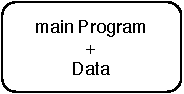
\includegraphics[width=0.20\textwidth]{images/01_1_non_structured_data.pdf}
    \caption{Programmazione non strutturata}
    \label{fig:nonstructured-programming}
\end{figure}

\subsubsection{Programmazione procedurale}
Il concetto base di questo tipo di programmazione è quello di raggruppare i pezzi di programma ripetuti in porzioni di codice utilizzabili e richiamabili ogni volta che se ne presenti l’esigenza. Le porzioni di codice con queste caratteristiche prendono il nome di \textit{procedure}. Ogni procedura può essere vista come un \textit{sottoprogramma che svolge una ben determinata funzione} e che è visibile e richiamabile dal resto del codice. La programmazione procedurale rappresenta un notevole passo in avanti rispetto a quella non strutturata, in quanto ne supera i limiti di ridondanza e garantisce una migliore gestione della memoria di sistema. Il vantaggio di una procedure sta nell'utilizzo dei parametri, allocati in memoria solo nel momento in cui una quest'ultima viene chiamata. Il \textit{main continua ad esistere} ma al suo interno presenta esclusivamente le invocazioni alle procedure definite dal programma. 
\begin{figure}[H]
    \centering
    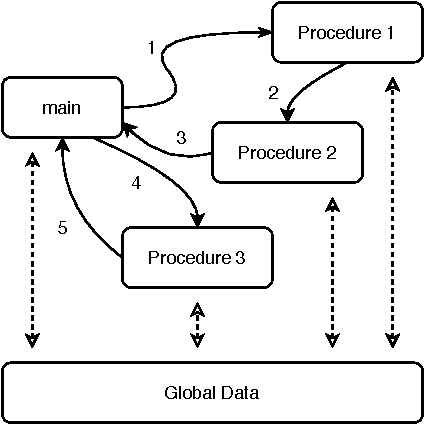
\includegraphics[width=0.50\textwidth]{images/01_2_procedural_programming.pdf}
    \caption{Programmazione procedurale}
    \label{fig:procedural-programming}
\end{figure}
Quando una procedura ha terminato il suo compito il controllo ritorna nuovamente al main (o alla procedura che ne ha effettuato l’invocazione) che esegue una nuova chiamata ad un’altra procedura fino alla terminazione del programma.

\subsubsection{Programmazione modulare}
Questo paradigma rapprenta un ulteriore passo avanti rispetto ai precedenti. La programmazione modulare risponde all'esigenza di poter \textit{riutilizzare le procedure messe a disposizione da un programma in modo che anche altri programmi ne possano trarre vantaggio}. L’idea alla base di questo paradigma è quella di raggruppare le procedure aventi un dominio comune (ad esempio, procedure che eseguono operazioni matematiche) in moduli separati. Quando si parla di \textbf{librerie di programmi}, in sostanza si fa riferimento proprio a moduli di codice indipendenti che ben si prestano ad essere riutilizzati in svariati programmi.
\begin{figure}[H]
    \centering
    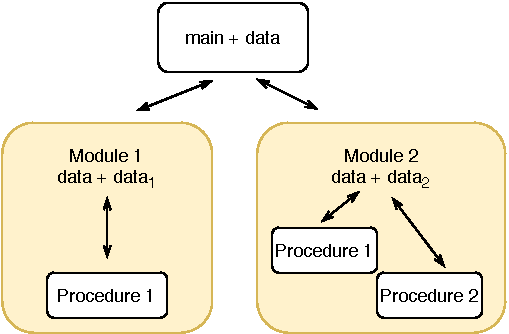
\includegraphics[width=0.50\textwidth]{images/01_3_modular_programming.pdf}
    \caption{Programmazione modulare}
    \label{fig:modular-programming}
\end{figure}
Con questo paradigma un singolo programma non è più costituito da un solo file (in cui è presente il main e tutte le procedure) ma da diversi moduli. Un singolo modulo può contenere anche dei dati propri che, in congiunzione ai dati del main, vengono utilizzati all’interno delle procedure in essi contenuti.

\subsection{Definizione}
\textit{Cosa si intende quindi quando si parla di programmazione a oggetti?} Con il termine programmazione orientata agli oggetti (da qui in seguito \textit{OOP}, in riferimento all'acronimo inglese) si pensa a un insieme di dati come a un singolo oggetto. Più oggetti possono interagire vicendevolmente, scambiandosi messaggi ma mantenendo ciascuno il proprio stato e i propri dati. Questa \textit{rivoluzione del metodo di programmazione} cambia l'approccio mentale all'analisi progettuale, ma non rinuncia ai vantaggi fino ad ora introdotti dai paradigmi precedenti, in particolare a quelli derivanti dall'utilizzo dei moduli. L’idea alla base di questo principio risiede, in buona parte, nel mondo reale. Un \textit{oggetto} è tipicamente un oggetto del mondo reale. In questo paradigma non ha importanza l'implementazione del codice ma, piuttosto, \textbf{le caratteristiche e le azioni} che un componente software è in grado di svolgere e che mette a disposizione di altri oggetti.  
\begin{figure}[H]
    \centering
    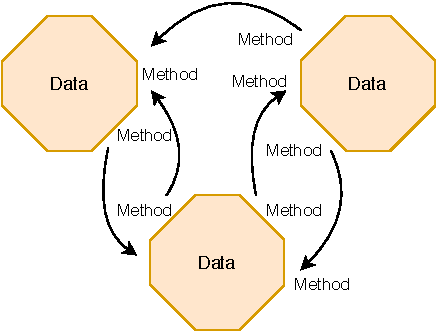
\includegraphics[width=0.50\textwidth]{images/01_4_object_oriented_programming.pdf}
    \caption{Colloquio tra oggetti}
    \label{fig:objectoriented-programming}
\end{figure}
Nella figura gli oggetti sono rappresentati dagli esagoni, che contengono i dati e comunicano attraverso metodi. Nella OOP, i dati (o caratteristiche dell'oggetto), prendono il nome di \textbf{proprietà}, mentre le azioni che essi possono fare \textbf{metodi}. Le proprietà vengono utilizzate dai metodi per eseguire determinate operazioni. Con l'espressione \textbf{pensare “ad oggetti”} quindi si identificano gli oggetti che entrano in gioco nel programma che si vuole sviluppare, gestendone l’interazione degli uni con gli altri.

\subsection{Java | Oracle}
\setlength{\epigraphwidth}{.6\textwidth}
\epigraph{<<The fact that you know Java doesn’t mean that you have the ability to transform that knowledge into well-designed object oriented systems>>}{Paul R. Reed}.\cite{reed:developingapplications}

La nascita del linguaggio Java alla fine del XX secolo segnò un punto di svolta per la programmazione a oggetti. La prima grande rivoluzione introdotta da questo linguaggio fu quella di liberare il programmatore dall'onere della gestione della memoria, che prima era gestita mediante l'utilizzo dei puntatori. Grazie a un sistema chiamato \textbf{garbage collector}, Java è in grado di assegnare e rilasciare automaticamente la memoria in base alla gestione del programma. La seconda rivoluzione introdotta è legata alla Java Virtual Machine (JVM), grazie alla quale i programmi non sono più compilati in codice macchina, ma in una sorta di linguaggio macchina “intermedio” (chiamato bytecode) che non è destinato ad essere eseguito direttamente dall’hardware ma che deve essere, a sua volta, interpretato da un secondo programma, la macchina virtuale appunto. In questo modo lo stesso codice può essere eseguito su più piattaforme semplicemente trasferendo il bytecode (non il sorgente) purché sia disponibile una JVM. Questo concetto prende il nome di \textbf{WORA}, \textit{write once, run everywhere}. Java fu incorporato da diversi web browser per permettere l'utilizzo delle \textit{applet}, un'applicazione che può essere avviata dall'utente eseguendo il codice scaricato da un server web remoto. 

\paragraph*{Perché Java?} Il linguaggio di programmazione è stata la prima decisione per un'ottimale azione di refactoring dell'applicazione e Java si è dimostrato essere il migliore per l'obiettivo dell'elaborato. Il rifacimento del backend è il primo passo sulla strada che porterà Zerocoda a un'evoluzione con conseguente inserimento in un panorama più ampio. Per questo motivo, la quasi totale indipendenza di Java dalla piattaforma hardware di esecuzione è una necessità chiave per l'applicazione, che così acquisisce una maggiore scalabilità. 

\subsubsection{La popolarità}
Prendendo in analisi i grafici offerti da \emph{TIOBE Programming Community Index} \cite{jansen:tiobe}, Java sembrerebbe essere al primo posto. Si tratta di un linguaggio facilmente manutenibile e dotato di molta documentazione che ne facilita l'apprendimento. Con le diverse librerie e framework compatibili è diventato il linguaggio di programmazione a oggetti più utilizzato al mondo, primo anche al precursore C++, dove la gestione della memoria e la curva di apprendimento possono rappresentare un problema. Java è stato adottato per la realizzazione del backend di diversi siti web di rilievo, come il sito d'asta e vendita online \textit{Ebay.com}.

\subsubsection{Le motivazioni}
Uno dei più grandi vantaggi offerti da questo linguaggio è proprio la sua capacità di addattamento ad aggiornamenti e modifiche del software in corso d'opera. Per capire meglio il perchè di questa scelta, facciamo riferimento al seguente esempio:
\begin{figure}[H]
    \centering
    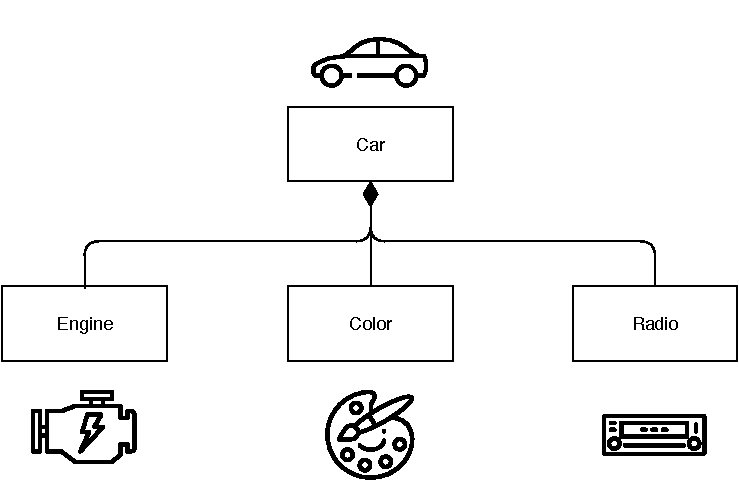
\includegraphics[width=0.75\textwidth]{images/01_5_java_class_diagram.pdf}
\end{figure}
Si pensi ad un rivenditore di auto che ha vari veicoli nel suo parco mezzi. Ogni veicolo è un \texttt{oggetto}, ma ognuno ha caratteristiche diverse denominate \texttt{classi}, che nel nostro esempio sono i diversi modelli, motori, colori della carrozzeria\dots Un cliente sceglie una macchina rossa, ma desidera aggiungere un impianto stereo migliore. La nuova macchina erediterà tutte le caratteristiche dell'oggetto "car" lasciando al programmatore il compito semplificato di modificare solamente la classe “radio” piuttosto che costruire da capo l’intero veicolo. Questo è ciò che rende Java la piattaforma ideale per i telefoni cellulari, i siti web, le console di gioco e qualsiasi applicazione che richieda aggiornamenti e modifiche frequenti.

%%%%%%%%%%%%%%%%%%%%%%%%%%%%%%%%%%%%%%%%%%%%%%%%%%%%%%%%%%%%%%%%%%%%%%%%%
\section{Database Relazionali}
Nello svolgimeto di ogni attività, sia a livello individuale sia in organizazioni di ogni dimmensione, sono essenziali la disponibilità di informazioni e la capacità di gestirle in modo efficiente. \cite{book:basididati} Un database relazionale è un tipo di database di archiviazione che fornisce accesso a data points tra i quali sussistono relazioni predefinite e che soddisfa queste esigenze. I database relazionali sono basati sul modello relazionale, un modello di rappresentazione dati semplice e diretto basato sull'utilizzo di tabelle.

\subsection{Modello Relazionale}
Il modello relazionale si basa su due concetti: \textbf{relazione} e \textbf{tabella}. La nozione di \textit{relazione} proviene dalla matematica, in particolare dalla teoria degli insiemi, mentre il concetto di \textit{tabella} è intuitivo. Il punto di forza del modello di database relazionale è l'uso delle tabelle, che permettono di archiviare informazioni strutturate e accedervi, risultando comprensibili anche per gli utenti finali.
\begin{table}[H]
    \centering
    \begin{tabular}{ |p{2cm}||p{2cm}|p{2cm}|p{3cm}|  }
        \hline
        Matricola & Cognome & Nome & Data di nascita\\
        \hline
        276545 & Rossi & Maria & 25/11/1996\\
        485745 & Neri & Fabio & 23/04/1997\\
        \hline
    \end{tabular}
\end{table}
\begin{table}[H]
    \centering
    \begin{tabular}{ |p{2cm}||p{2cm}|p{2cm}|  }
        \hline
        Studente & Corso & Voto\\
        \hline
        276545 & Analisi & 28\\
        485745 & Chimica & 27\\
        \hline
    \end{tabular}
\end{table}
\begin{itemize}
    \item l'ordine delle colonne e delle righe all'interno di una tabella è insignificante
    \item non possono esistere due righe identiche, ogni riga può essere contrassegnata con un identificatore univoco (chiave principale) che ne faciliti la distinzione dalle altre
    \item  ogni colonna in una tabella ha un nome univoco e contiene un solo tipo di dato
    \item un campo (o cella) può contenere un solo valore effettivo di un attributo
    \item le righe di tabelle diverse possono essere correlate utilizzando chiavi esterne
\end{itemize}

\subsection{Struttura}
Secondo il modello relazionale, le strutture dei dati logici, ovvero tabelle di dati, viste e indici, sono separate dalle strutture di storage fisiche. Grazie a questa separazione, gli amministratori di database possono gestire lo storage fisico dei dati senza compromettere l'accesso a tali dati come struttura logica. Questo permette di accedere ai dati in modi diversi senza riorganizzare le tabelle e di ottenere quindi \textbf{l'indipendenza fisica dei dati}.

\subsection{Database non Relazionali}
Questo tipo di struttura dati si differenzia da quella appena presentata dal momento che non richiede uno schema fisso. La base su cui poggia tutta la costruzione dei database di questo tipo non è costituita da tabelle di dati ma da documenti. La forza di questo principio è proprio che tutto quello che serve all’applicazione risiede nel documento già precompilato. Si evita le frammentazione dell’informazione e la sua ricostruzione, con i rischi di perdere dati o averne di corrotti. Un aumento di flessibilità che velocizza le operazioni e offre risposte più veloci all'utente finale.
\begin{figure}[H]
    \centering
    \begin{minted}{JSON}
        {
            "276545" : {
                "cognome" : "Rossi",
                "nome" : "Maria",
                "data_di_nascita" : "25/11/1996",
                "esami" : [
                    {
                        "corso" : "Analisi",
                        "voto" : 28,
                    }
                ]
            },
            "485745" : {
                "cognome" : "Neri",
                "nome" : "Fabio",
                "data_di_nascita" : "23/04/1997",
                "esami" : [
                    {
                        "corso" : "Chimica",
                        "voto" : 27,
                    }
                ]
            },
        }
    \end{minted}
    \caption{Esempio di documento di un database non relazionale}
    \label{fig:nonrelational-database}
\end{figure}

\subsection{Le differenze}
Un database non relazionale (chiamato anche \textit{NoSQL}) è preferibile quando si ha a che fare con una grande quantità di dati. Questa sua struttura, molto aperta ad aggiunte e scalabile orizzontalmente, rappresenta una grande fattore di rischio per un problema che nei database relazionali è gestito in maniera ottimale: la duplicazione dei dati. Un aspetto che tuttavia depone a favore dei database non relazionali lo si trova nell'\textbf{inserimento dei dati}. Se da una parte per i database NoSQL l'inserimento dei dati risulta più facile e privo di rischi, per i database relazionali un cattivo inserimento può portare alla corruzione dei legami tra tabelle, e quindi all'ottenimento di dati poco edificabili. 

\subsubsection{Integrità dei dati} 
Con un database NoSQL è possibile costruire un documento adatto alla mappatura delle classi-oggetto del proprio applicativo riducendo di molto i tempi di sviluppo. La \textit{mancanza dei controlli fondamentali sull'integrità dei dati}, tuttavia, delega all'applicativo che dialoga con il database questo compito, che ovviamente dovrà essere testato in maniera più approfondita prima di essere messo in produzione. Nei database relazionali questo tipo di controllo avviene all'interno dello stesso database. 

\subsection{MySQL}
Quotidianamente, immense quantità di informazioni vengono affidate a tecnologie che ne garantiscono la conservazione duratura ed un recupero efficiente che ne permetta l’analisi. Da anni, questo ruolo viene interpretato molto bene da un prodotto software completo, efficiente ed affidabile: MySQL. Questo software è un DBMS (database management system) open source per la gestione di database relazionali e rappresenta una delle tecnologie più note e diffuse nel mondo dell'IT. I programmi che dovranno interagire quindi con una base di dati non potranno farlo direttamente, ma dovranno dialogare con il DBMS, che sarà l’unico ad accedere fisicamente alle informazioni.
\begin{figure}[H]
    \centering
    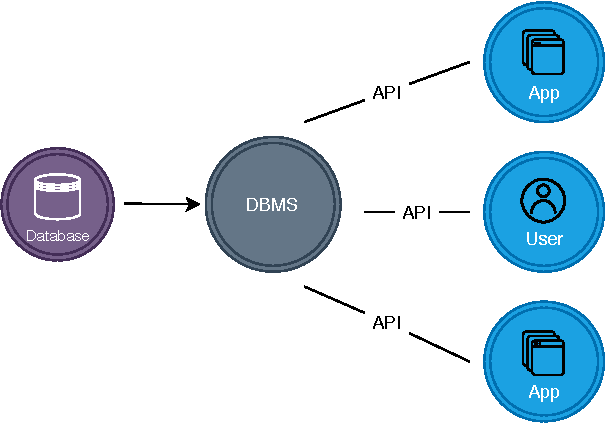
\includegraphics[width=0.65\textwidth]{images/01_6_dbms.pdf}
    \caption{Database management system}
    \label{fig:databasemanagementsystem}
\end{figure}
Oltre alla gestione del database, un DBMS deve controllarne l'accesso concorrente, assicurarne la sicurezza e l'integrità dei dati e permetterne la condivisione e l'integrazioni con applicazioni differenti. Grazie a queste caratteristiche le applicazioni che vengono sviluppate possono contare su una sorgente dati sicura, affidabile e generalmente scalabile.

\subsubsection{Il linguaggio SQL}
Il nome SQL deriva l’abbreviazione di \textit{Structured Query Language}, un linguaggio di programmazione che consente di accedere e gestire i dati in un database relazionale. Questo linguaggio rappresenta lo \textbf{standard per database basati sul modello relazionale}. La diffusione di SQL è dovuta in buona parte alla intensa opera di standardizzazione dedicata a questo linguaggio, svolta principalmente nell'ambito degli organismi ANSI (\textit{American national Standards Institute}, l'organismo nazionale statunitense degli standard) e ISO (l'organismo internazionale che coordina i vari organismi nazionali).

\paragraph{Funzionalità e Sintassi} A seconda dell'operazione che si vuole eseguire sul database, SQL mette a disposizione diverse tipologie di linguaggi:
\begin{itemize}
    \item \textit{DDL - Data Definition Language} per creare e modificare \texttt{schemi di database}
    \item \textit{DML - Data Manipulation Language} inserire, modificare e gestire dati memorizzati
    \item \textit{DQL - Data Query Language} per interrogare i \texttt{dati memorizzati}
    \item \textit{DCL - Data Control Language} creare e gestire strumenti di controllo e accesso ai dati
\end{itemize}
Sarebbe quindi diminutivo definire SQL 'un semplice linguaggio di interrogazione' in quanto alcuni dei suoi sottoinsiemi sopra elencati permettono di creare, gestire e modificare il database. La popolarità di SQL è inoltre dovuta alla sua facilità di comprensione, dovuta a un linguaggio con comandi semplici, autoesplicativi nella loro sintassi, e prestante per qualsiasi tipo di operazione.
\begin{figure}[H]
    \centering
    \begin{minted}{SQL}
        SELECT Matricola, Cognome, Nome, Corso, Voto 
        FROM Studenti JOIN Esami 
        ON Matricola = Studente
    \end{minted}
    \caption{Esempio di query SQL}
    \label{fig:sql-example}
\end{figure}
\begin{table}[H]
    \centering
    \begin{tabular}{ |p{2cm}||p{2cm}|p{2cm}|p{2cm}|p{2cm}|  }
        \hline
        Matricola & Cognome & Nome & Corso & Voto\\
        \hline
        276545 & Rossi & Maria & Analisi & 28\\
        485745 & Neri & Fabio & Chimica & 27\\
        \hline
    \end{tabular}
\end{table}

%%%%%%%%%%%%%%%%%%%%%%%%%%%%%%%%%%%%%%%%%%%%%%%%%%%%%%%%%%%%%%%%%%%%%%%%%

\section{Architettura di Microservizi}
\subsection{Architettura Monolitica}
Ai primordi dello sviluppo applicativo, anche un cambiamento minimo  a un software esistente imponeva un aggiornamento completo e un ciclo di controllo qualità. Le applicazioni erano sviluppate e distribuite come una singola entità, e tale approccio veniva spesso definito \textbf{“monolitico”}, perché il codice sorgente dell’intera applicazione era compilato in una singola unità di deployment. 

\begin{figure}[H]
    \centering
    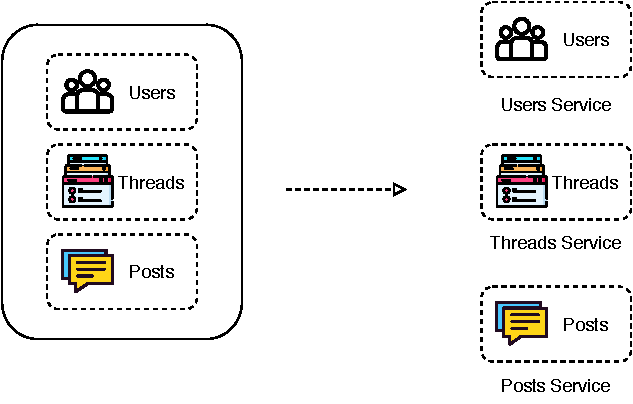
\includegraphics[width=0.75\textwidth]{images/01_7_monolithic_vs_microservices.pdf}
    \caption{Architettura Monolitica e Microservizi }
    \label{fig:monolithicvsmicroservices}
\end{figure}

\paragraph{Caratteristiche} Le applicazioni che seguono questo tipo di architettura sono di facile implementazione, in quanto tipicamente raccolte all'interno di un unico progetto e distribuite in un unico pacchetto. Questo tipo di architettura si presta bene per applicazioni piccole o comunque poco soggette a cambiamenti, ma la cosa cambia quando ci troviamo a sviluppare applicazioni complesse che richiedono continui aggiornamenti. Se uno di questi dovesse causare errori, l'unica soluzione sarebbe quella di \textit{disconnettere tutto} e fare un rollback totale del software: è chiaro che un'azienda non può permettersi tempi di inattività. L’unico modo di poter scalare un’applicazione monolitica è quello di replicare l’intera applicazione con conseguente aumento di costi e risorse necessarie. In seguito ai problemi derivanti da questo tipo di architettura, nacquero i primi studi di archittetture a servizi, sulla base di uno dei dogmi dell'ingegneria del software:

\newtheorem*{defin1}{Principio di Singola Responsabilità}
\begin{defin1}
    Riunire le cose che cambiano per lo stesso motivo e separare quelle che cambiano per motivi diversi.
\end{defin1}

\subsubsection{Cosa sono i Microservizi}
L'architettura di microservizi rappresenta un'approccio all'avanguardia per lo sviluppo e l'organizzazione del software. Secondo questo stile, il software è composto da servizi indipendenti di piccole dimensioni che hanno come finalità lo svolgimento di un unico compito, e di farlo nel migliore dei modi. \cite{amazon:microservices} Ciascun microservizio, indipendente dagli altri, è dunque gestito da un unico team di sviluppo. Per una definizione più precisa riprendiamo le parole di Martin Fowler, considerato uno dei massimi esperti in materia, che afferma: \textit{<<Lo stile architetturale a microservizi è un approccio allo sviluppo di una singola applicazione come insieme di piccoli servizi, ciascuno dei quali viene eseguito da un proprio processo e comunica con un meccanismo snello, spesso una HTTP API.>>} \cite{fowler:microservices}

\subsection{Le origini}
Il primo tentativo di architettura a servizi nasce con l’\texttt{architettura SOA}. Il concetto delle \textit{Service-Oriented Architecture} si afferma all’inizio degli anni Duemila come una collezione di servizi indipendenti che comunicano gli uni con gli altri tramite un \textit{Enterprise Service Bus (ESB)}. L’architettura a microservizi è una chiara \textbf{evoluzione dell’architettura SOA}, spinta dall’esigenza  di una sempre più’ marcata scalabilità, la quale permette di reggere il carico di milioni di utenti connessi in un determinato istante.

\subsection{Le differenze con SOA}
Per studiare le differenze tra le due architettura facciamo riferimento al seguente schema:
\begin{figure}[H]
    \centering
    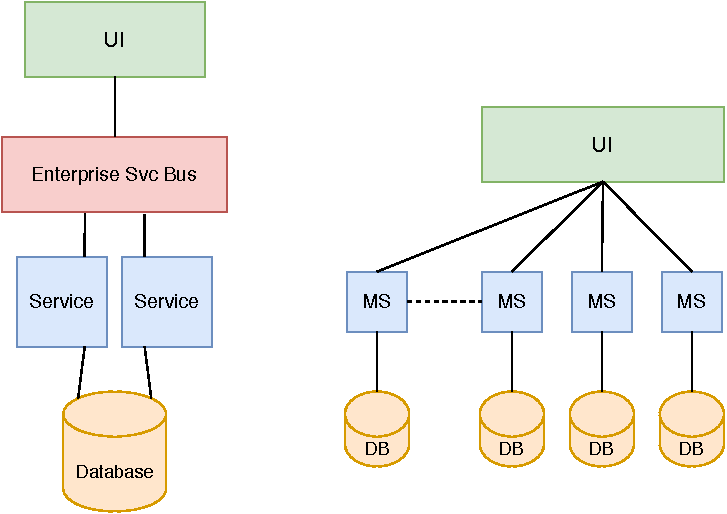
\includegraphics[width=0.80\textwidth]{images/01_8_microservices_vs_soa.pdf}
    \caption{Architettura SOA e Microservizi }
    \label{fig:soavsmicroservices}
\end{figure}
\paragraph*{Granularità dei Servizi} Il numero dei servizi è un buon fattore per la differenziazione delle due architetture. Lo stesso Martin Fowler, citato precedentemente, afferma che in un'architettura SOA non si arriva neanche ad una decina di  servizi mentre in un architettura a microservice il numero dei servizi e’ molto più alto: basti pensare che il servizio di streaming Netflix ha dichiarato di fare uso di oltre di 700 microservizi. \cite{article:netflixmicroservices}

\paragraph{Comunicazione} I microservizi abbandonano l’utilizzo di ESB, comunicando direttamente tra loro con meccanismi di comunicazione light. Nella SOA, l’ESB potrebbe diventare un singolo punto di errore che influisce sull’intero sistema. Poiché ogni servizio comunica attraverso l’ESB, se uno dei servizi rallenta, potrebbe ostruire l’ESB con le richieste per quel servizio. D’altra parte, i microservizi sono molto migliori nella tolleranza agli errori: se un microservizio presenta un errore di memoria, verrà interessato solo quel microservizio.

\paragraph{Database} In SOA i servizi condividono gli storage mentre con i microservice ogni servizio può avere un database indipendente.

\subsection{Caratteristiche dei Microservizi}

\subsubsection{Autonomia}
Ciascun servizio nell’architettura basata su microservizi può essere sviluppato, distribuito, eseguito e ridimensionato senza influenzare il funzionamento degli altri componenti. I servizi non condividono alcun codice o implementazione con gli altri.

\subsubsection{Specificità}
Ciascun servizio è progettato per una serie di capacità e si concentra sulla risoluzione di un problema specifico. Se nel tempo si decide di rendere un servizio più complesso, il servizio può essere scomposto in servizi più piccoli.

\subsubsection{Eterogeneità delle Tecnologie}
Durante lo sviluppo di un microservizio si ha totale libertà di scelta nell'utilizzo delle tecnologie. Ciascuna tecnologia viene decisa esclusivamente in base allo scopo del microservizio, senza basarsi sulla sua interazione con gli altri. Un microservizio può fare affidamento su un modello di database relazionale mentre un servizio con cui comunica su uno di tipo non relazionale, così come la loro logica può essere scritta in linguaggi differenti.

\subsubsection{Semplicità di Distribuzione}
Con i microservizi è possibile apportare una modifica a un singolo servizio e distribuirlo indipendentemente dal resto del sistema con tecniche di continuos delivery del tutto automizzate. Questo permette di rilasciare aggiornamenti più velocemente e in maniera più sicura.

\subsubsection{Resilienza}
La resilienza è la capacità di accettare la possibilità’ di errori e continuare a funzionare. Con i microservizi, le applicazioni possono gestire completamente gli errori di un servizio isolando la funzionalità senza bloccare l’intera applicazione.

\subsubsection{Scalabilità}
I microservizi consentono di scalare ciascun servizio in modo indipendente per rispondere alla richiesta delle funzionalità che un'applicazione supporta. 

%%%%%%%%%%%%%%%%%%%%%%%%%%%%%%%%%%%%%%%%%%%%%%%%%%%%%%%%%%%%%%%%%%%%%%%%%

\section{Web Services e API}

\subsubsection{Cos'è un Web Service}
Secondo la definizione data dal World Wide Web Consortium (W3C), si definisce \emph{Web Service} un \textsc{sistema software} che si mette al servizio di un'applicazione ed è progettato per supportare l'interoperabilità tra diversi elaboratori sulla medesima rete. \cite{w3c:webservices} Il servizio web è in grado di offrire un’\textit{interfaccia software} comprendente un file WSDL (Web Services Description Language) che descrive il servizio in modo più dettagliato. Il client può utilizzare il file WSDL per capire quali funzioni può svolgere sul server tramite le operazioni esposte dall'interfaccia, e in che modo le richieste devono essere costruite. Infine, la comunicazione funziona attraverso diversi protocolli e architetture. 

\subsubsection{Cos'è un'API}
Un'\textit{Application Program Interface (API)} può essere considerata come un \textsc{contratto} tra un fornitore di informazioni e l'utente destinatario di tali dati: l'API si limita a stabilire il contenuto richiesto dal consumatore (la chiamata) e il contenuto richiesto dal produttore (la risposta). Un'API funge quindi da elemento di intermediazione tra gli utenti e le risorse che questi intendono ottenere. È anche un mezzo con il quale un'organizzazione può condividere risorse e informazioni assicurando al contempo sicurezza e controllo, poiché stabilisce i criteri di accesso. L'utilizzo di un'API permette all'utente di rimanere all'oscuro delle specifiche con cui le risorse vengono recuperate o della loro provenienza.
\begin{figure}[H]
    \centering
    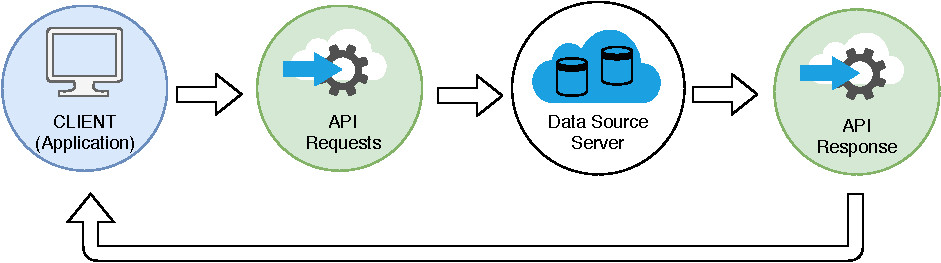
\includegraphics[width=0.90\textwidth]{images/01_9_api.pdf}
    \caption{Funzionamento delle API}
    \label{fig:api}
\end{figure}

\subsection{Representational State Transfer - REST}
Il Representational State Transfer è lo stile architetturale più popolare degli ultimi anni. Non si tratta di un protocollo nè tantomeno di una specifica (in quanto non fa riferimento a uno standard ufficiale), ma piuttosto di una serie di vincoli per la creazione di un servizio web che può servirsi di standard,  come HTTP, URI, JSON e XML. REST permette di \textit{accedere} e \textit{modificare} la \textbf{rappresentazione testuale di risorse}, attraverso una serie di \textbf{operazioni stateless} \textit{uniformi} e \textit{predefinite}. Generalmente basato su HTTP, permette di utilizzare anche altri protocolli di trasferimento come SNMP, SMTP, ecc\dots

\paragraph{Perchè è conveniente?} L'utilizzo di API Rest fornisce una notevole quantità di libertà e flessibilità agli sviluppatori. Questo stile architetturale non richiede l'installazione di alcuna libreria (fatta eccezione per HTTP Client-Server e il JSON parser). Non vincola  chi lo sceglie a utilizzare una tecnologia, ma al contrario ne supporta diverse.

\paragraph{Cosa la rende semplice?} L'informazione, o rappresentazione, viene consegnata in uno dei diversi formati tramite HTTP: JSON (Javascript Object Notation), HTML, XLT o testo semplice. Il formato JSON è uno dei più diffusi, perché indipendente dal linguaggio e facilmente leggibile da persone e macchine.
\begin{figure}[H]
    \centering
    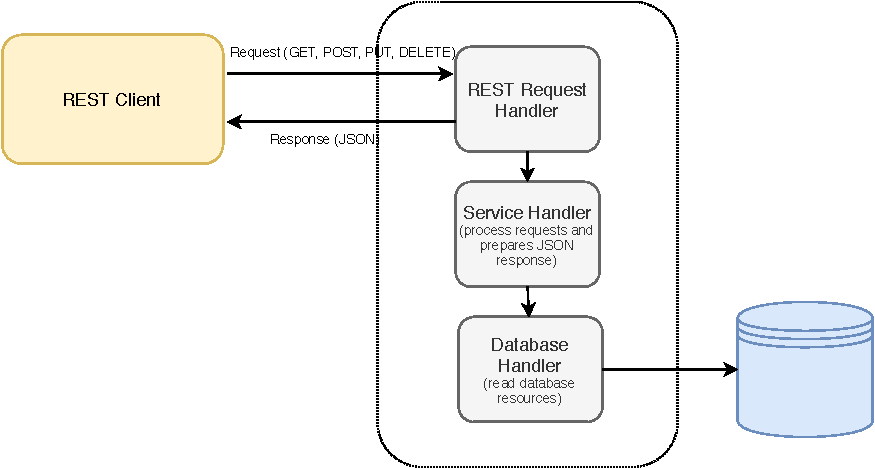
\includegraphics[width=0.95\textwidth]{images/01_10_restapi.pdf}
    \caption{Funzionamento delle API Rest}
    \label{fig:restapi}
\end{figure}
\begin{figure}[H]
\begin{minted}{HTML}
    GET /messages HTTP/1.1
    Host: domainname.com
    Content-Type: text/plain;charset:UTF-8
    Content-Length: 44
\end{minted}
\caption{Esempio di Richiesta REST}
\label{fig:restrequest}
\end{figure}

\subsubsection{Principi REST}
Di seguito esponiamo i \textit{sei principi per un'architettura REST}, per la prima volta introdotti durante la dissertazione nella tesi di dottorato di Roy Fielding, uno dei principali autori delle specifiche dell'Hypertext Transfer Protocol (HTTP). \cite{fielding:restprinciples}

\paragraph{1. Client-Server} Secondo questo principio, nello sviluppo di un'architettura REST Client e Server devono rimanere separati, in modo da potersi evolvere individualmente. Per questo motivo, si dice che rispetta il paradigma dell'informatica noto come \textbf{Separation of Concerns (SoC)}, traducibile in italiano come \emph{suddivisione dei compiti}. Secondo il principio SoC il sistema deve essere diviso in moduli distinti, ciascuno dedito allo svolgimento di un proprio compito, supportando in tal modo l’evoluzione indipendente della logica lato client e della logica lato server. Secondo questo vincolo il server deve offrire una o più funzionalità e ascoltare le richieste di possibili client. Un client deve invocare il servizio messo a disposizione dal server inviando il corrispondente messaggio di richiesta. Il servizio lato server a questo punto respinge la richiesta o esegue l’attività richiesta prima di inviare un messaggio di risposta al client. La gestione delle eccezioni è delegata al client.

\paragraph{2. Stateless} Con questo termine si fa riferimento al tipo di operazioni. Le singole invocazioni delle API Rest non devono fare affidamento alle risorse presenti sul server, ma esclusivamente sui dati forniti nella stessa richiesta. Nel client non è previsto un sistema di memorizzazione delle informazioni delle richieste, ciascuna di queste è distinta e non connessa. Ciò garantisce una forte scalabilità, riducendo l'utilizzo di memoria sul server.

\paragraph{3. Cache} Le Rest API devono essere progettate in modo da favorire l'utilizzo di date cachable. \emph{La richiesta di rete più efficiente è quella che non utilizza la rete.} In un 'architettura REST i messaggi di risposta dal servizio ai suoi consumatori sono esplicitamente etichettati come memorizzabili nella cache oppure non memorizzabili. In questo modo, il servizio, il consumatore o uno dei componenti intermediari possono memorizzare nella cache la risposta per il riutilizzo nelle richieste successive. Le richieste vengono passate attraverso un componente cache, che può riutilizzare le risposte precedenti per eliminare parzialmente o completamente alcune interazioni sulla rete.

\paragraph{4. Interfaccia Uniforme} Il Client deve essere in grado di comunicare con il server usando un singolo linguaggio, indipendentemente dall'architettura di backend. Questo permette alle informazioni di essere trasferite in una forma standard.

\begin{itemize}
    \item \textbf{Identificazione delle Risorse} Una risorsa è un oggetto o la rappresentazione di qualcosa di significativo nel dominio applicativo. Il concetto di risorsa è quindi molto simile a quello di oggetto nel mondo della programmazione ad oggetti.
    \item \textbf{Manipolazione delle risorse attraverso rappresentazioni} Una risorsa può essere rappresentata in molti modi diversi. Ad esempio come HTML, XML, JSON o anche come file JPEG. I client interagiscono con le risorse tramite le loro rappresentazioni, il che è un modo potente per mantenere i concetti di risorse astratti dalle loro interazioni.
    \item \textbf{Hypermedia come motore dello stato dell’applicazione} L’applicazione deve essere guidata da collegamenti, consentendo ai clienti di scoprire risorse tramite collegamenti ipertestuali.
\end{itemize}

\paragraph{5. Sistema a strati} In un sistema a livelli, componenti intermedi come i proxy possono essere collocati tra client e server.
Uno dei vantaggi di un sistema a più livelli è che gli intermediari possono intercettare il traffico client-server per scopi specifici; ad esempio il caching, la sicurezza o l'autenticazione. Una soluzione basata su REST può essere composta da più livelli architettonici indipendenti l’uno dall’altro.

\paragraph{6. Codice su richiesta} Vincolo opzionale. Richiede che il codice eseguibile possa essere trasmesso su richiesta creando un'applicazione che non dipende più esclusivamente dalla propria architettura. I problemi di sicurezza e l'eterogeneità dei linguaggi di programmazione tuttavia costituiscono un limite per l'adozione di questo vincolo.

\subsection{Simple Object Access Protocol - SOAP}
SOAP è un protocollo ufficiale gestito dal W3C (World Wide Web Consortium), ideato inizialmente per consentire la comunicazione tra applicazioni realizzate con linguaggi e piattaforme diverse. Trattandosi di un protocollo, richiede l'integrazione di regole che ne aumentano la complessità e il carico di gestione sul sistema, comportando tempi di caricamento delle pagine più lunghi. Oltre alle regole, integra anche standard di conformità che lo rendono idoneo agli ambienti enterprise. Oltre alla sicurezza, gli standard di conformità integrati includono: 
\begin{itemize}
    \item \textsc{atomicità}
    \item \textsc{coerenza}
    \item \textsc{isolamento}
    \item \textsc{durata}
\end{itemize}
Dal loro acronimo l'insieme di questi standard prende il nome di \textbf{ACID}.

\subsubsection{Richieste e Risposte}
Una richiesta di dati inviata a un'API SOAP può essere gestita tramite uno dei protocolli a livello applicativo: HTTP (per i browser web), SMTP (per l'email), TCP e altri. Una volta ricevuta la richiesta, i messaggi SOAP di ritorno devono essere restituiti come documenti in formato \textbf{XML}, un linguaggio di markup facilmente leggibile da utenti e macchine. Una \textit{richiesta completata a un'API SOAP non viene memorizzata nella cache del browser}, e pertanto non sarà possibile accedervi successivamente senza rinviarla all'API.

\begin{figure}[H]
    \begin{minted}{XML}
        <soap:Envelope xmlns:soap="http://schemas.xmlsoap.org/soap/envelope/">
            <soap:Body>
                <getProductDetails xmlns="http://domainname.com/ws">
                <productId>827635</productId>   <!-- ID della risorsa -->
                </getProductDetails>
            </soap:Body>
        </soap:Envelope>
    \end{minted}
    \caption{Esempio di Richiesta SOAP}
    \label{fig:soaprequest}
\end{figure}


\subsubsection{Differenze con REST}
La differenza sostanziale tra le due tecnologie introdotto risiede nel fatto che SOAP è un protocollo con requisiti specifica, contrariamente a REST che è un insieme di linee guida con implementazione flessibile. Molti sistemi esistenti aderiscono ancora a SOAP, mentre REST, il cui avvento è successivo, è spesso considerato come un'alternativa più rapida negli scenari web. Poiché sono ottimizzate, le API REST sono adatte ai contesti più innovativi come l'Internet of Things (IoT), lo sviluppo di applicazioni mobili e il serverless computing. Grazie all'integrazione della sicurezza e della conformità delle transazioni, i servizi web SOAP rispondono a molte esigenze aziendali, ma risultano anche più complessi.
\chapter{Architettura Funzionale del Sistema}
\label{chap:systemdesign}
In questo capitolo è illustrato il funzionamento del sistema prima e dopo l'azione di refactoring, presentando le tecnologie che utilizza e accennando alle soluzioni pensate per ogni specifico problema. Vengono presentate l'architettura del sistema di partenza e quella di arrivo, in riferimento al modello di sviluppo dell'\emph{ingegneria del software} seguito.
\section{Funzionamento dell'Applicazione}
\subsection{Scenario}
Lo scopo di quest'applicazione è quello di \textit{velocizzare l'accesso ai servizi sanitari}. Senza questo \textit{primo requisito}, l'applicazione non troverebbe posto nel mondo enterprise. Per questo motivo, l'interfaccia utente risulta semplice e comprende poche funzionalità. 
\paragraph{L'utente} per accedere ai servizi deve registrarsi al sistema fornendo i propri dati personali (che potranno essere modificati in qualsiasi momento), scegliendo un'email e una password per le future autenticazioni. Anche senza essere registrato può cercare una struttura tra quelle presenti e scegliere un servizio che questa eroga. 
\paragraph{I servizi} possono essere diversi: analisi, esami, visite mediche, qualsiasi servizio che preveda un'attesa del cliente potrebbe essere inserito da una struttura sanitaria. Selezionando un servizio, all'utente viene mostrato il relativo calendario di disponibilità, in termini di giorni e fasce orarie. 
\paragraph{La prenotazione} avviene una volta selezionato un orario (corrispondente a uno \emph{slot}) e confermata l'intenzione di volerlo riservare. Per fare quest'operazione è necessario che l'utente sia autenticato al sistema. Prima di confermare la prenotazione di uno slot, l'utente può scegliere se inserire i dati (almeno uno tra nome e cognome, email o telefono) di un altro utente, anche non iscritto al sistema, per cui prenotare il servizio. Scegliendo questa opzione il destinatario sarà informato mediante delle notifiche sui futuri eventi relativi allo stato della sua prenotazione. A questo punto all'utente viene fornito un ``biglietto virtuale'', che è univoco per quel determinato servizio.
\paragraph{Il biglietto} consiste in una numerazione. Questa numerazione corrisponde al numero che verrà chiamato allo sportello (si pensi ad un biglietto virtuale staccato al momento della prenotazione). Ciascun servizio è identificato da una lettera dell’alfabeto (A, B, C, \dots) mentre ciascun numero identifica il cliente in coda (1, 2, 3, \dots). In questo modo la numerazione B12, ad esempio, fa riferimento al cliente numero 12 di un servizio, C13 ad un altro cliente di un altro servizio. L’idea è che chi ha prenotato si presenti presso la struttura nel momento esatto in cui viene erogato il servizio, evitando coda e assembramenti. In questo modo anche la logistica dietro a un servizio può essere ottimizzata, ad esempio preparando i documenti necessari alla visita.
\paragraph{La struttura } deve avere informazione di questo biglietto virtuale, così come l’utente.  Questo avviene attraverso un \textsl{software} installato in loco che prende il nome di \textbf{MRU}, dal nome di Mauro e Ruggero, i due ideatori del sistema software.
\paragraph{L'MRU} è un software che disponde di un'interfaccia web per gli operatori e per i totem che vengono utilizzati. Tutte le notti l'MRU interroga Zerocoda richiedendo le prenotazioni per la giornata odierna. Se queste sono presenti le scarica. In questo modo anche gli operatori hanno informazione delle prenotazioni.

\subsection{Use Case Diagram}
In Figura \ref{fig:zerocodausecase} è presentato il diagramma dei casi d'uso di un utente generico di Zerocoda. I diversi colori utilizzati per le operazioni che l'utente può fare rappresentano la \textit{divisione in servizi} scelta per la fase di implementazione delle REST API.
\begin{figure}[H]
    \centering
    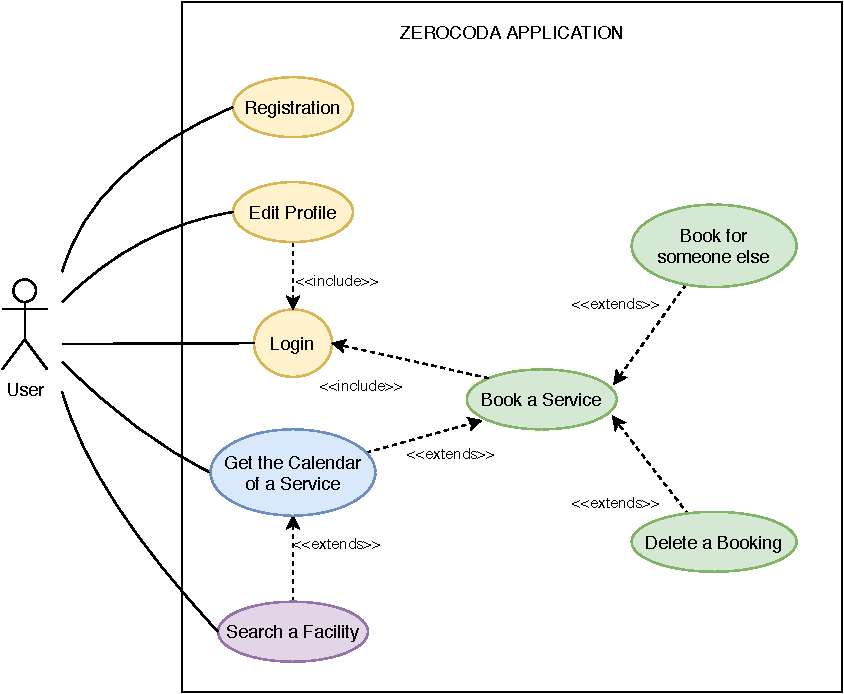
\includegraphics[width=0.95\textwidth]{images/02_1_zerocoda_usecase.pdf}
    \caption{Zerocoda Use Case Diagram}
    \label{fig:zerocodausecase}
\end{figure}

\subsection{I diversi Enti Zerocoda}
Sull'applicazione Zerocoda è possibile prenotare i servizi erogati da diversi enti. Alcuni di questi, tuttavia, non sono presenti sul sito. Ci sono strutture sanitarie che non vogliono che i loro utenti accedano a un sito generalista come \emph{Zerocoda.it}. Questi vogliono che il loro sito funga da ``vetrina'', che l'utente riconosca la struttura presso cui prenota attraverso elementi come il logo, il nome, ecc. L'utilizzo del \textbf{virtual hosting} risponde a questa esigenza. In fase di accesso il servizio compare come se fosse erogato dell’ente privato. Questi \textit{siti premium} consistono in realtà in un sito statico (come lo stesso Zerocoda), ma con una configurazione dedicata, che una volta ricevuta dal browser cambia il \emph{look and feel}.

\paragraph{É possibile offrire una  personalizzazione maggiore} ai siti che la richiedono. La richiesta può spaziare dall'utilizzo di colori particolari per gli elementi della pagina: quali pulsanti, form, colori del background, a quella di immagini e loghi personalizzati o alla necessità di avere funzionalità esclusive rispetto ad altre strutture.

\paragraph{La configurazione} consiste in un file JSON contenente tutte le informazioni del sito. Oltre alle informazioni relative al nome, indirizzo, descrizione, questo file contiene anche stringhe di testo già formattate in HTML, da inserire all'interno della pagina in appositi spazi. Può contenere anche informazioni riguardanti lo stile (CSS) della pagina. La configurazione viene caricata per ultima, dopo che i componenti statici sono stati renderizzati. Viene inviata al frontend attraverso uno script JavaScript.

%%%%%%%%%%%%%%%%%%%%%%%%%%%%%%%%%%%%%%%%%%%%%%%%%%%%%%%%%%%%%%%%%%%%%%%%%
\section{Analisi dell'Applicazione}
Gli attuali clienti (enti sanitari) per Zerocoda sono 45. Il numero comprende sia gli enti presenti su Zerocoda, sia coloro che hanno richiesto una personalizzazione su un proprio portale. Il sistema, in totale vanta i seguenti numeri:
\begin{itemize}
    \item 1 Zerocoda
    \item 17 siti con configurazione personalizzata
    \item 500.000 utenti registrati
    \item 298 impianti di MRU registrati
\end{itemize}


\subsection{Multitenancy}
La particolarità del sistema è quella di essere \textbf{multitenant} (Figura \ref{fig:multitenancy}). Con un solo servizio è possibile offrire esperienze isolate agli utenti: una diversa esperienza sulla base della loro organizzazione. In questo modo, se un nuovo ente richiedesse che tutti i suoi dati fossero salvati su un nuovo database, si potrebbe installare un nuovo ambiente separato apposito. In alcuni casi è possibile anche chiedere metodi di registrazione o accesso al sistema ad-hoc, evitando il sistema standard basato su email e password. Così facendo, il sistema si limiterebbe ad esporre un'API in aggiunta all'applicazione condivisa da tutti, che gestisce la richiesta di autenticazione personalizzata sulle necessità dell'ente richiedente.
\begin{figure}[H]
    \centering
    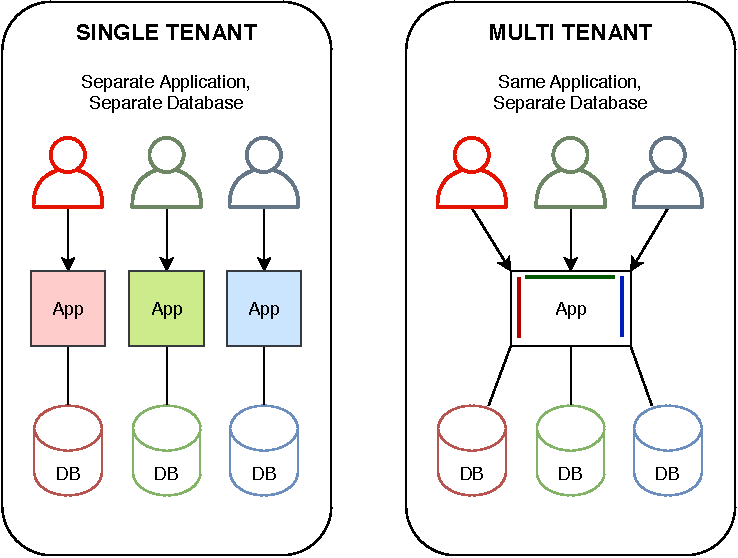
\includegraphics[width=0.94\textwidth]{images/02_2_multitenancy.pdf}
    \caption{Single Tenant vs. Multi Tenant}
    \label{fig:multitenancy}
\end{figure}

\subsection{Backend Overview}
Ad oggi non è presente un elemento definibile come \emph{layer di API} nell’applicazione. Il sistema è composto da un unico monolite che tra le tante mansioni che ha espone anche le `API'. Nello stesso sistema viene effettuato ogni genere di controllo per quanto rigurarda l'autenticazione e i parametri passati nelle richieste. Il backend è interamente scritto in PHP e si appoggia ad un database MySQL. Nonostante con gli ultimi aggiornamenti PHP offra la possibilità di programmare a oggetti, questo non è il caso del sistema preso in analisi. Per la creazione di dati che in altri linguaggi sarebbero rappresentabili attraverso oggetti, il backend utilizza un sistema di liste con elementi di tipo chiave-valore.

\subsection{Chiamate delle API}
Le chiamate dal frontend alle API intercettano il click sul documento, andando a cercare il componente su cui è stata registrata l'interazione. Tutte le richieste inviate al backend sono richieste GET HTTP. Quindi, passando un qualsiasi parametro o effettuando operazioni di aggiunta o modifica di dati, i parametri vengono aggiunti all'URL, e mostrati in chiaro. Questo scelta è stata adottata anche per i metodi di registrazione e autenticazione, i più delicati dal punto di vita della sicurezza. Con la sintassi \texttt{\$\_GET} in PHP si fa riferimento a una variabile globale che contiene i parametri in GET della richiesta HTTP.
\begin{figure}[H]
\begin{alltt}
    \centering
    http://domain.it/index.php/api/v1/login?
    \centering
    _apikey=1&
    email=mariarossi2020%40studenti.unipr.it&
    password=Password123!
    callback=jQuery22404905003978295608_1605812447764&
    _=1605812447767
\end{alltt}
\caption{Esempio di richiesta GET in HTTP}
\label{fig:getlogin}
\end{figure}
Prendendo in analisi la richiesta di login in Figura \ref{fig:getlogin}, nell'url sono presenti i parametri \textsl{email} e \textsl{password} utilizzati per autenticare l'utente. Questi dati sensibili \textit{non dovrebbero appartenere all'url} dove sono visibili, ma andrebbero passati nel \emph{body} di una richiesta. Con la variabile \texttt{\$\_GET} in PHP è dunque possibile accedere anche a questi parametri.

\subsubsection{Scenario}
Il sistema, per capire quale API è stata chiamata, ricerca il metodo della richiesta passando il parametro \texttt{\$\_GET} all'interno di un costrutto condizionale di grandi dimensioni e verificando ogni chiamata possibile. In Figura \ref{fig:apicall} viene presentata una ricostruzione di parte del codice a cui si fa riferimento. Quando il valore del parametro corrisponde al nome del metodo chiamato, nello stesso ciclo richiama l'operazione richiesta. Risulta facile notare che il codice, implementato in questo modo, presenta diversi lati negativi. Vengono ripetute parti di codice, i parametri vengono istanziati dentro ciascun \emph{if statement} e passati ai metodi che ne richiedono l'utilizzo: tutto questo all'interno della stessa condizione. Infine, i risultati di ciascuna chiamata vengono istanziati all'interno di array.
\usemintedstyle{pastie}
\begin{figure}
    \inputminted[firstline=2, lastline=15]{octave}{src/examples/old_api_call.php}
    \caption{Struttura delle chiamate Api}
    \label{fig:apicall}
\end{figure}

\subsection{Same Origin Policy}
Un'origine è definita da un \textit{protocollo}, un \textit{dominio} e una \textit{porta} di un URL. Più in generale, i documenti appartenenti a pagine web differenti sono isolati gli uni dagli altri. L'intento di questa politica è quello di consentire l'accesso a siti non sicuri, ma senza che quest'ultimi abbiano la possibilià di interferire con la sessione di chi naviga su un sito sicuro. \cite{w3c:sop}

\paragraph{I controlli} di origine vengono applicati dal browser in ogni caso di potenziale interazione tra elementi di origini diverse. Questo include, ma non è limitato a:
\begin{itemize}
    \item Codice JavaScript e Document Object Model (DOM)
    \item Cookies
    \item Chiamate AJAX (XmlHTTPRequest)
\end{itemize}

\subsubsection{Chiamate AJAX}
L'\emph{Asynchronous JavaScript and XML} è ad oggi la tecnica più utilizzata per sviluppare applicazioni web interattive. Il concetto che sta alla base di una chiamata AJAX è quello di \textit{poter scambiare dati tra client e server senza ricaricare la pagina}: lo scambio avviene in background tramite una chiamata asincrona dei dati di solito utilizzando l’oggetto \textsl{XMLHttpRequest}. Il framework \textbf{jQuery} semplifica notevolmente l'implementazione di chiamate di questo tipo, e a ciò deve la sua fama.

\subsubsection{Cross Origin Resource Sharing - CORS}
In alcuni casi, lavorare con domini differenti che interagiscono tra loro può rivelarsi \textit{una necessità}. Quando ciò accade, \textit{è possibile allentare la Same Origin Policy} in modo che non ostacoli le funzionalità di interazione tra domini dell’applicazione web. Ciò può essere fatto in diversi modi, ad esempio: dichiarando l'origine utilizzando JavaScript, l'intestazione di una chiamata, o stabilendo un sistema di autenticazione tra le due parti. Questa procedura prende il nome di \textit{Cross-Origin Resource Sharing}. L'utilizzo di questo meccanismo fa a caso nostro per quanto riguarda le chiamate delle API di Zerocoda, le quali si trovano su un dominio differente rispetto a quello della pagina web. Siccome durante il primo sviluppo dell'applicazione non si aveva pensato ad una soluzione simile, durante la nuova fase di analisi si è tenuto conto di questo aspetto. Nell'implementazione si lavorerà dunque alla stesura di API su un differente dominio, garantendone l'accesso e dichiarando affidabili le origini necessarie. Alla nascita di Zerocoda si è elaborato un modo per aggirare questo problema, piuttosto che eliminarlo alla radice.

\subsubsection{JSONP}
JSONP è l’acronimo di \emph{JSON with Padding} ed è la tecnica utilizzata per ovviare alla limitazione imposta dalla Same Origin Policy. Il suo funzionamento di base è semplice: permette a un browser di accedere a risorse remote mediante codice JavaScript, indipendentemente dall’host di origine. La tecnica permette di invocare una \textit{funzione di callback} automatizzata (come spesso viene fatto per le richieste AJAX basate su XmlHttpRequest) al ricevimento di dati. Il JSON è definito all'interno di questa funzione. Al caricamento del file JavaScript, l'interprete esegue la funzione di callback, che è così in grado di restituire il JSON al client.
\usemintedstyle{friendly}
\begin{figure}[H]
    \inputminted{octave}{src/examples/jsonp.js}
    \caption{JSONP Callback - Login}
    \label{fig:jsonpexample}
\end{figure}
Nella Figura \ref{fig:jsonpexample} viene presentata la callback utilizzata per restituire all'utente i propri dati dopo un'autenticazione andata a buon fine. La chiamata AJAX (invocata da JQuery) viene così mascherata con il caricamento di un file JavaScript. La stringa di numeri presente sul parametro callback viene inizializzata con un valore corrispondente al nome randomico di una funzione appena creata da uno script server-side. Come si osserva dalla precedente Figura \ref{fig:getlogin} il server ha conoscenza della funzione da andare a creare, in quanto ottiene questa informazione dai parametri del metodo GET utilizzato. Il codice JavaScript inserito nella pagina HTML utilizza poi questa funzione per passare i parametri che normalmente vengono restituiti con un file JSON. Si tratta sostanzialmente di un'invocazione di funzione.

%%%%%%%%%%%%%%%%%%%%%%%%%%%%%%%%%%%%%%%%%%%%%%%%%%%%%%%%%%%%%%%%%%%%%%%%%
\section{Architettura Precedente}
In Figura \ref{fig:oldarchitecture} viene rappresenta l'architettura del sistema \emph{precedente} al refactoring. Di seguito vengono analizzate le tecnologie che essa utilizza.
\begin{figure}[H]
    \centering
    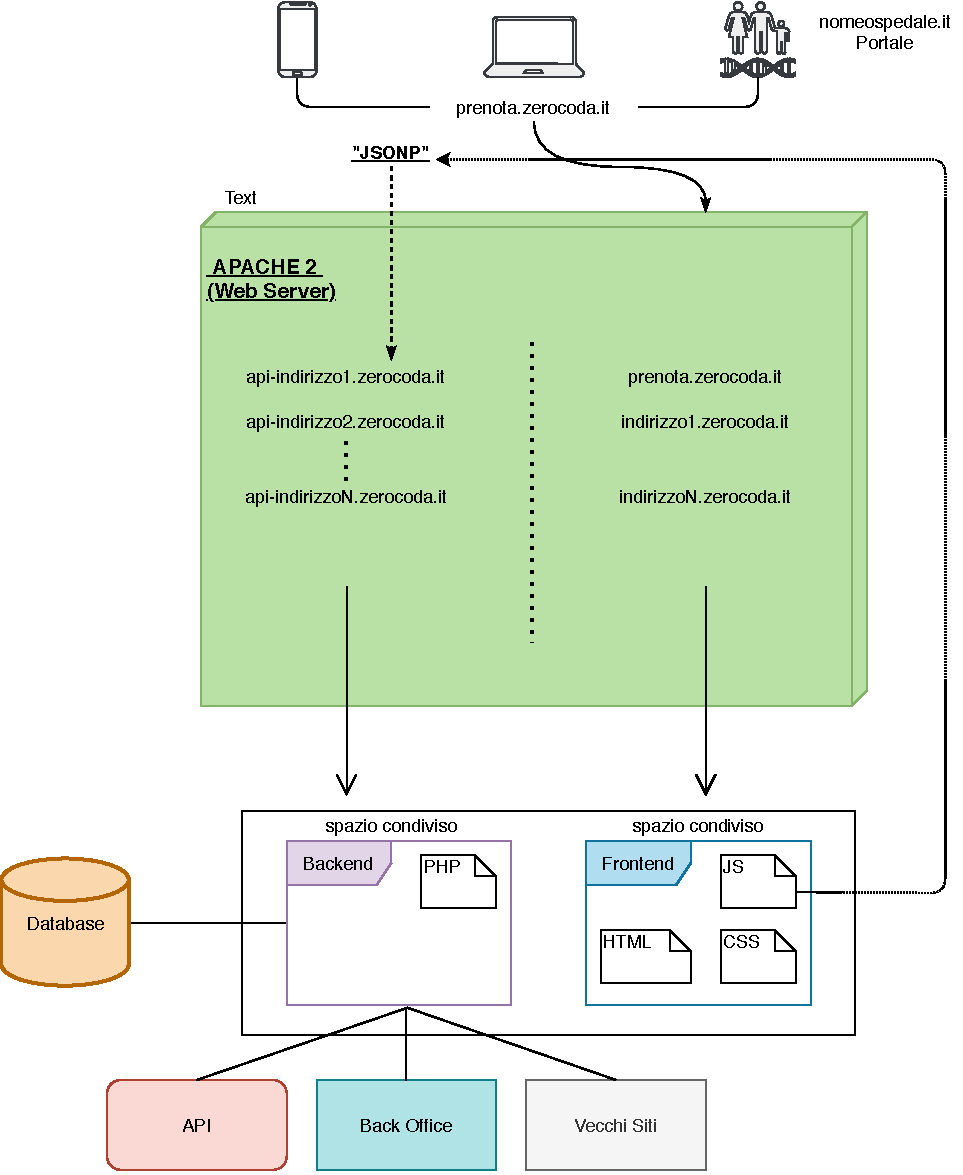
\includegraphics[width=0.95\textwidth]{images/02_3_old_architecture.pdf}
    \caption{Architettura del Sistema di Partenza}
    \label{fig:oldarchitecture}
\end{figure}

\subsection{Web Server Apache}
A livello di file system si ha uno spazio condiviso per il backend (interamente in PHP) e uno spazio condiviso per il frontend, contenente i soli contenuti statici (HTML, CSS e immagini). Il backend funge da colonna portante per diversi componenti:
\begin{itemize}
    \item \textbf{backoffice}: sostanzialmente l'interfaccia amministrativa di Zerocoda. Attraverso questa interfaccia è possibile gestire tutto il sistema. Viene utilizzata principalmente per aggiungere quelli che si definiscono 'slot', ma può essere anche utilizzata per creare e gestire utenti. Uno \emph{slot} è un posto prenotabile per un servizio in un determinato giorno e in una determinata fascia oraria. Con il backoffice un amministratore può aggiungere in modo semi-automatico gli slot per un determinato servizio, scegliendone il numero per ogni ora e lo stato (abilitato o disabilitato) al momento della creazione.
    \item \textbf{vecchi siti } precedenti al refactoring. Prima di questo refactoring il frontend del sito era stato aggiornato. Nulla è stato cambiato per quanto riguarda il funzionamento, solo gli elementi grafici sono stati modificati per rispondere ad uno stile più moderno. Nonostante ciò, si è scelto di mantenere online il frontend per alcuni siti, che in questo modo rimane sempre a carico di Apache.
    \item \textbf{API}: le chiamate esposte in precedenza. Le API a cui si fa riferimento quando si invia una richiesta per effettuare un'operazione sono le stesse per tutti i dispositivi. Non c'è differenza che si acceda da un browser web, un dispositivo mobile, o dal portale di un sito con configurazione personalizzata.
\end{itemize}   
Con le caratteristiche attuali Apache2 funziona esclusivamente da Web Server.

\subsection{Virtual Hosting}
Non tutti i siti hanno abbastanza traffico da giustificare il costo di un web server dedicato, pertanto la loro condivisione su un singolo web server può essere una buona soluzione per abbassarne il costo. Il \emph{virtual hosting} viene incontro a questa esigenza, permettendo ad un unico server web di “ospitare” più siti (e/o applicazioni) web, i quali condivideranno, secondo opportune politiche di gestione, le risorse di elaborazione del server stesso. Consolidare più servizi su un’unica macchina è una pratica comunemente adottata poiché permette di ottimizzare l’utilizzo delle risorse hardware disponibili. Senza il virtual hosting, si renderebbe necessario attivare una nuova macchina server per ogni nuovo sito o applicazione web, con un conseguente aumento dei costi ed un possibile sottoutilizzo delle risorse hardware. Con l'attuale architettura \textit{Apache ospita al suo interno una serie di virtual host}.

\paragraph{Funzionamento} Il server Apache, con un unico indirizzo IP, ospita più di un nome di dominio. I diversi domini, com'è  possibile osservare dalla Figura \ref{fig:virtualhosting} condividono la stessa porta, ma si può anche assegnare a ciascun dominio una porta specifica.

\begin{figure}[H]
    \centering
    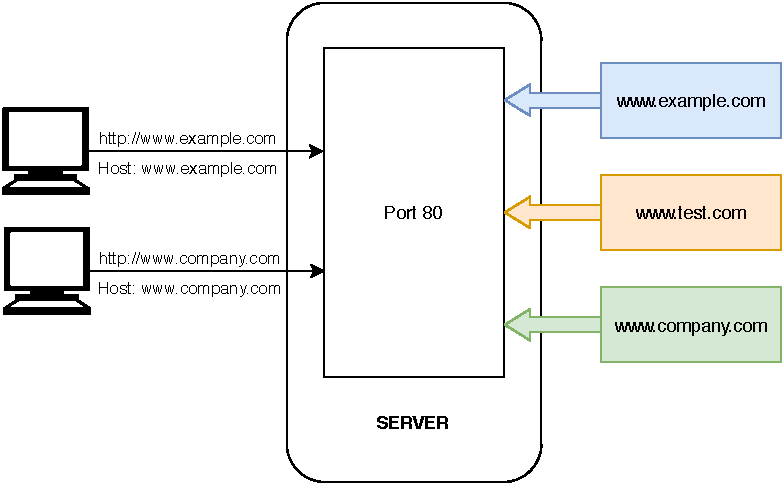
\includegraphics[width=0.98\textwidth]{images/02_4_virtual_hosting.pdf}
    \caption{Funzionamento del Virtual Hosting}
    \label{fig:virtualhosting}
\end{figure}

\subsection{Database MySQL}
Il dialogo con il database avviene attraverso il codice PHP del backend. È compito del server Apache fornirne l'accesso per una serie di indirizzi (le API). Il database è \textit{unico per tutti gli enti Zerocoda}, anche gli enti `premium' interrogano la stessa base di dati degli altri. Coloro che hanno richiesto un metodo di accesso diverso da quello standard si limitano ad avere una tabella isolata dagli altri, contenente i dati dei propri utenti. Poiché questa tipologia di enti ha gli utenti su una tabella diversa, avrà anche API apposite per interrogarla. Questa API si trova sempre all'interno dello stesso backend, insieme alle altre.

%%%%%%%%%%%%%%%%%%%%%%%%%%%%%%%%%%%%%%%%%%%%%%%%%%%%%%%%%%%%%%%%%%%%%%%%%
\subsection{Limiti del Database}
La struttura del database non corrisponde a quella che ci si aspetterebbe in un tipico sistema di prenotazioni utente. Nel database sono infatti contenute diverse tabelle di configurazione per il software, per lo più utilizzate nel backoffice in fase di amministrazione. Queste tabelle contengono ad esempio i giorni festivi all'interno di un anno (in cui non è quindi possibile prenotare determinati servizi), o i giorni della settimana per evitare prenotazioni errate nei weekend dove alcune strutture possono essere chiuse. Tra queste sono presenti anche tabelle per la configurazione dei campi utente in fase di registrazione e altre contenti i messaggi di errore da restituire. Questi tipi di tabelle vengono utilizzate quindi come metodo di controllo nelle query. Inoltre, sul database vengono salvati anche i log riguardanti il funzionamento dello stesso: è logico dedurre che, in caso di malfunzionamento, non c'è modo di verificare questi documenti.

\subsubsection{Autenticazione}
 Per autenticarsi l'utente fornisce la propria email e la propria password, che, al momento del primo accesso, contribuiscono alla generazione di un token casuale da parte del sistema. Per gli accessi successivi questo stesso token viene utilizzato per identificare l'utente. In principio Zerocoda era sprovvista di un sistema di autenticazione mediante token randomici. Questa funzionalità è stata introdotta poco prima del refactoring, tuttavia i token di autenticazione vengono salvati sul database e interrogati dallo stesso backend piuttosto che da un server esterno. Nella progettazione della nuova architettura si è pensato a questo problema, gestendolo attraverso un apposito microservizio.

\subsubsection{Verifica delle API Keys}
Non è presente nessuna struttura intermediaria tra client e server che si occupi di fare i controlli necessari per la verifica delle API Keys, pertanto queste operazioni si traducono in delle semplici query alla base di dati. L'API Key deve essere un \emph{campo obbligatorio} nella richiesta di un'operazione. Questa permette di identificare l'ente/i corrispondenti, mostrandone i relativi dati sulla pagina. Ad esempio, un utente che accede a Zerocoda deve essere in grado di vedere i soli enti e servizi corrispondenti ad un'API Key, mentre accedendo ad un portale di un sito con una propria configurazione deve vedere i soli dati relativi a prenotazioni e servizi di quella struttura. Anche il controllo dell'Api Key, come per l'autenticazione, si è deciso di delegarlo a un nodo intermedio.

\subsubsection{Ridondanza dei Dati}
Come le precedenti, anche la ridondanza dei dati è un limite che ha dato diversi problemi durante la manutenzione del software. Il database presenta due tabelle con lo stesso scopo: \textit{users} e \textit{bookers}. Inizialmente le due erano state pensate con compiti diversi. La prima avrebbe registrato i dati degli \emph{amministratori di sistema}, coloro che hanno necessità di accedere al backoffice, mentre la seconda avrebbe contenuto i dati degli \emph{utenti finali} di Zerocoda. La continua manutenzione degli ultimi anni ha portato il software ad essere sviluppato sempre da \textit{persone diverse}. Questo, unito all'ambiguo nome dato a tabelle, ha portato i dati ad essere incosistenti da quelli pensati nel disegno orginale. Al momento, i dati di un utente in fase di registrazione vengono quindi salvati su due tabelle distinte.

\subsubsection{Vincoli di Integrità}
I vincoli di integrità permettono alle tabelle di disporre di \emph{regole rigide} riguardanti i dati che è possibile inserire al loro interno. Il database non le utilizza in tutte le tabelle. Il modo in cui i dati vengono inseriti o eliminati dal database deve essere sempre lo stesso e coerente negli anni. Non essendo così, anche i metodi di interrogazione ne risentono. Un sistema di questo tipo dovrebbe avere poche query, semplici e comprensibili, tuttavia la disuguaglianza di alcuni valori all'interno del database non lo rende possibile. Alcune prenotazioni, eliminate da utenti o amministratori, presentano valori \emph{null}, mentre altre hanno il valore `0' che le identifica come `non prenotate'. Quando è necessario eliminare un dato presente su più tabelle, spesso occorre fare più di una query, controllandone il risultato. Questi problemi si sarebbero potuti evitare in fase di progettazione.
%%%%%%%%%%%%%%%%%%%%%%%%%%%%%%%%%%%%%%%%%%%%%%%%%%%%%%%%%%%%%%%%%%%%%%%%%
\section{Reingegnerizzazione}
\newtheorem*{def:reverseengineering}{Definizione}
\begin{def:reverseengineering}
    La reingegnerizzazione è quel processo di esame, analisi e alterazione di un sistema software esistente, col fine di ricostruirlo in una nuova forma, e la successiva implementazione. \cite{chikofsky:reverseengineering} Nel processo di reingegnerizzazione è compresa anche la riprogettazione del software, mentre quando si parla di reverse engineering si fa riferimento all'analisi.
\end{def:reverseengineering}
Il reverse engineering del codice permette di invertire i processi di sviluppo e produzione di un software e quindi di ottenere uno sguardo prezioso dietro le quinte di un programma. Attraverso lo studio dettagliato del codice sorgente è possibile comprendere, riscrivere o ricostruire l’architettura di un programma, il suo funzionamento e le sue strutture interne. Apparentemente la reingegnerizzazione non dovrebbe essere fatta per modificare i requisiti funzionali del sistema. In realtà, spesso quando si applica questa tecnica ci si accorge, in fase di riprogettazione, che alcuni requisiti, dopo anni di sviluppo, non sono più validi e andrebbero tolti dal disegno, mentre altri, nuovi, andrebbero introdotti.

\subsection{I motivi}
La pandemia di quest'ultimo anno ha portato l'azione di refactoring su \emph{Zerocoda} ad essere a tutti gli effetti una necessità. Il distanziamento sociale è un bisogno per ogni tipo servizio offerto ad una clientela più o meno vasta, e tenere traccia dei clienti e del loro numero temporizzando gli accessi al servizio è senza alcun dubbio la soluzione migliore. Nello stato attuale, tuttavia, l'applicazione non rispetta i requisiti funzionali per essere rilasciata ad un pubblico di tipo \emph{enterprise}. Sono sempre di più le aziende che hanno richiesto l'inserimento dei loro servizi nell'applicazione. L'inserimento di nuovi servizi porterebbe all'aumento delle richieste da parte dei client, più richieste a più dati da elaborare, e più dati a un sovraccarico. L'applicazione non è pronta a uno scenario di questo tipo, pertanto urge un refactoring mirato all'introduzione di nuove tecnologie, che renda il software più scalabile in prevenzione del nuovo numero di clienti sulla piattaforma.

Questo rappresenta il motivo principale, quello che ha portato l'azione di refactoring, dapprima solo ipotizzata da coloro che già lavoravano al sistema, a un inizio di progettazione. Normalmente le esigenze possono essere anche altre:

\begin{itemize}
    \item il team di sviluppo è cambiato e sono subentrati altri programmatori che non hanno conoscenze in merito al sistema;
    \item la documentazione è assente del tutto o, se presente, dopo anni di sviluppo e modifiche non è stata aggiornata e risulta obsoleta;
    \item  l'introduzione di piccoli cambiamenti risulta complessa e costosa da affrontare in termini di tempo e risorse;
    \item il software è spesso soggetto a continue correzioni di bug, indice che la struttura è precaria e mal progettata;
    \item numerose correzioni sono state apportate e si è verificato il fenomeno dell' `architectural drift' (deriva architetturale), cioè il sistema si è spostato molto dal disegno originale che non è più chiaro;
    \item i metodi e gli strumenti di sviluppo originali sono ormai superati ed è difficile trovare programmatori con queste conoscenze.
\end{itemize}

%%%%%%%%%%%%%%%%%%%%%%%%%%%%%%%%%%%%%%%%%%%%%%%%%%%%%%%%%%%%%%%%%%%%%%%%%
\section{Modello di Sviluppo}
Come \textit{metodologia di sviluppo} si è scelto di adottarne una di tipo \textbf{agile}. Secondo questo \emph{principio teorico}, il punto di partenza è costituito dalla specifica dei requisiti, mentre lo sviluppo vero e proprio del software avviene solo in seguito.

\subsection{Waterfall Model}
Il modello a cascata è un \textbf{ciclo di vita lineare}, che suddivide il processo di sviluppo in fasi di progetto consecutive. A differenza dei modelli iterativi, \textit{ogni fase viene eseguita solo una volta}. Con questo modello il progetto viene organizzato in una sequenza di fasi, ciascuna delle quali produce un output che costituisce l’input per la fase successiva.

\subsubsection{Origini}
Lo sviluppo del modello viene attribuito allo scienziato informatico Winston W. Royce, che tuttavia, non è stato il suo vero inventore. Al contrario, il suo articolo pubblicato nel 1970 “Managing the Development of Large Software Systems” \cite{royce:softwaredevelopment} conteneva una critica aperta nei confronti dei cicli di vita lineari. Come alternativa, presentava un modello iterativo-incrementale, in cui ogni fase attinge a quella precedente e ne verifica i risultati. 

\paragraph{Il modello di Royce} è cosituito da sette fasi eseguite in diversi passaggi (iterazioni):

\begin{enumerate}
    \item Requisiti di sistema
    \item Requisiti di software
    \item Analisi
    \item Progettazione
    \item Implementazione
    \item Test
    \item Esecuzione e Manutenzione
\end{enumerate}
Il modello a cascata si ispira alle fasi definite da Royce, ma prevede solo un’iterazione.

\subsubsection{Funzionamento}
Nella pratica vengono utilizzate diverse versioni del modello a cascata. Attualmente vengono utilizzati dei modelli che suddividono i processi di sviluppo in cinque fasi. Le fasi 1, 2 e 3, definite da Royce, sono riunite in un’unica fase di progetto, chiamata analisi dei requisiti. (Figura \ref{fig:waterfallmodel})
\begin{enumerate}
    \item Analisi: pianificazione, analisi e specificazione dei requisiti
    \item Progettazione: progettazione e specificazione del sistema
    \item Implementazione: programmazione e test di modulo
    \item Test: integrazione di sistema, test di sistema e test di integrazione
    \item Esecuzione: rilascio, manutenzione, miglioramento
\end{enumerate}
\begin{figure}
    \centering
    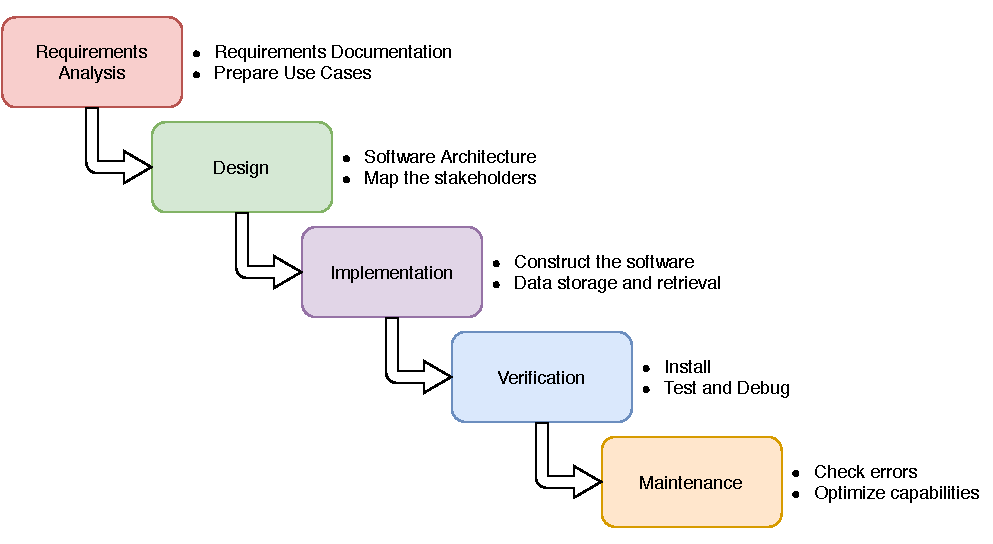
\includegraphics[width=0.98\textwidth]{images/02_5_waterfall_model.pdf}
    \caption{Fasi del Modello a Cascata}
    \label{fig:waterfallmodel}
\end{figure}
Il modello da noi utilizzato rappresenta un'\textit{estensione del modello a cascata}, in quanto l'eseguire ogni fase una sola volta comporta un grande vincolo. Ad ogni fase infatti si confrontano e verificano i risultati ottenuti con quelli della fase precedente. Partendo da un'analisi delle esigenze richieste dall'applicazione, dai suoi limiti e dalle necessità dei clienti, si è poi passati all'individuazione di una strada per lo sviluppo.

%%%%%%%%%%%%%%%%%%%%%%%%%%%%%%%%%%%%%%%%%%%%%%%%%%%%%%%%%%%%%%%%%%%%%%%%%
\section{Nuova Architettura}
\begin{figure}[H]
    \centering
    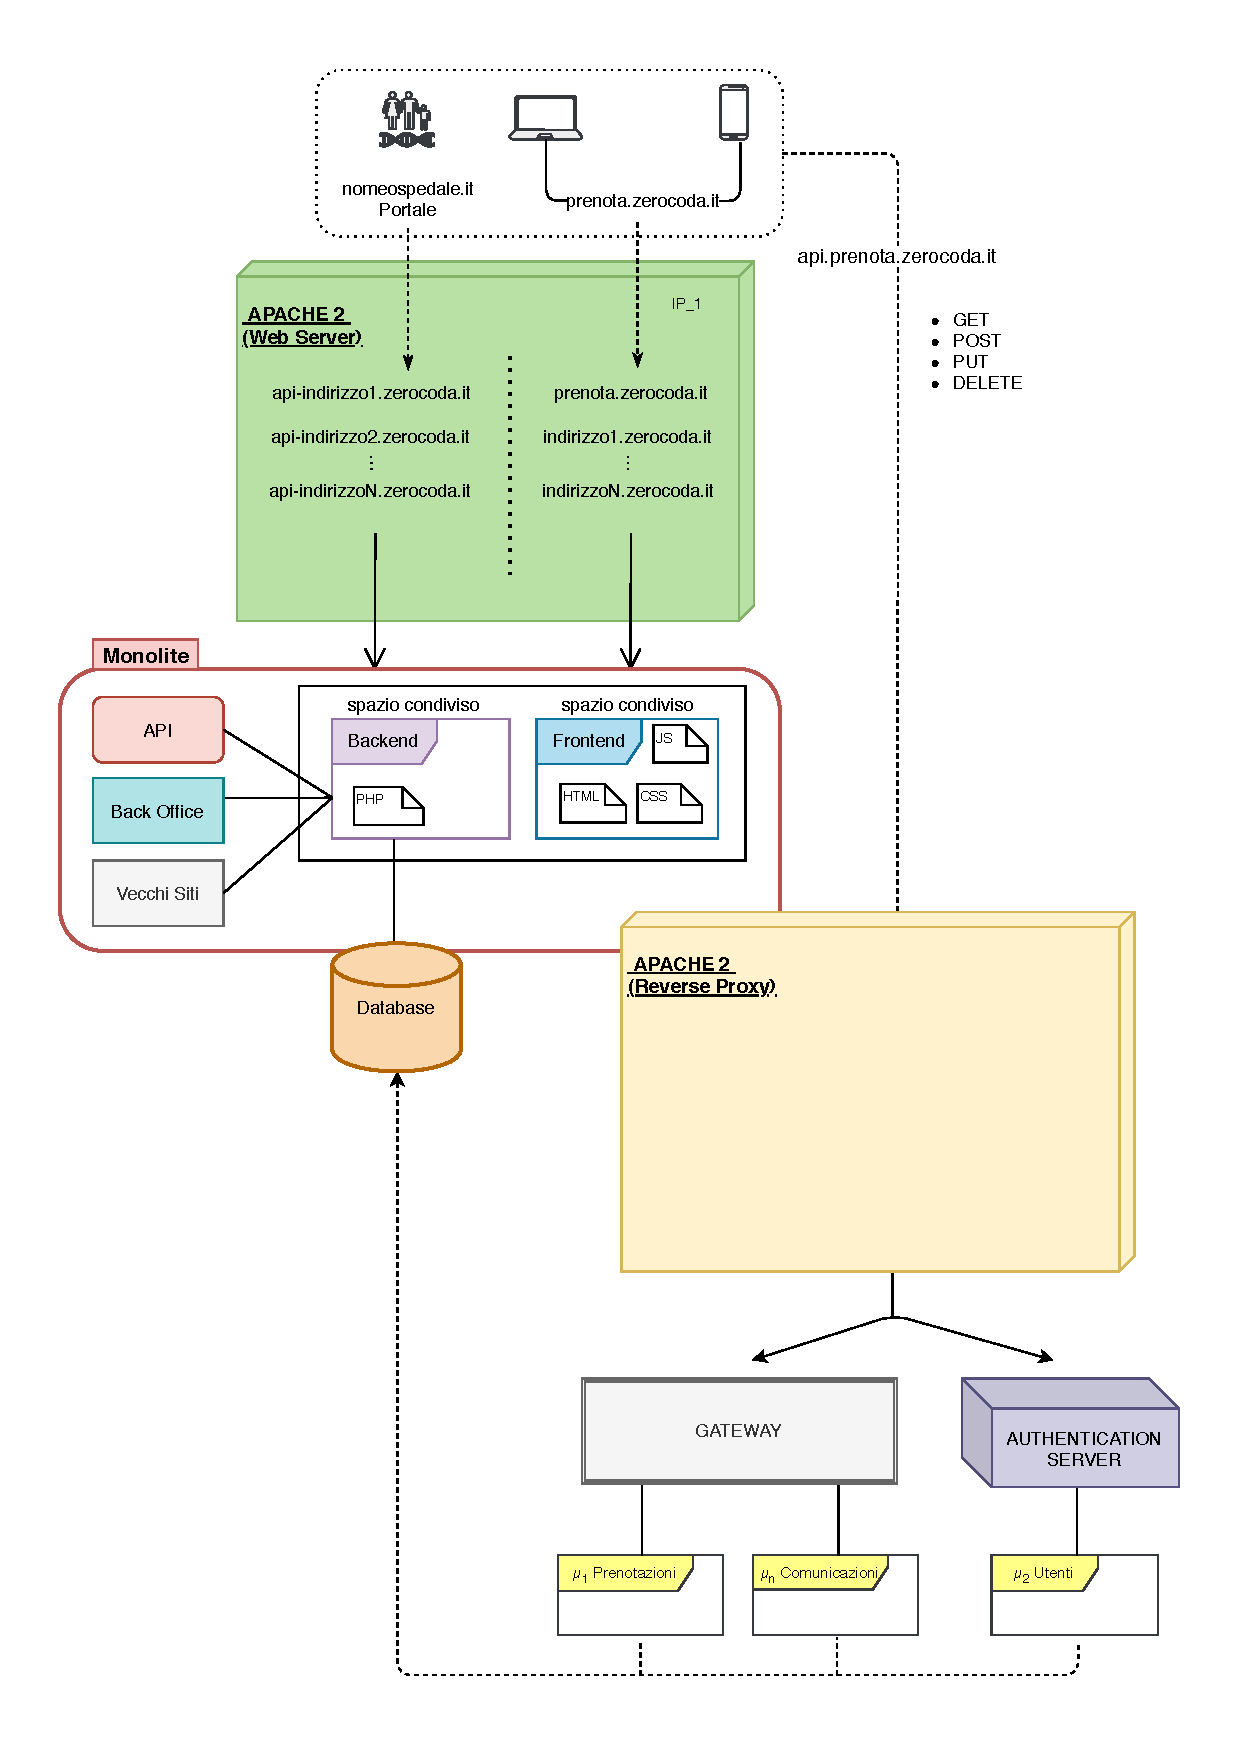
\includegraphics[width=0.86\textwidth]{images/02_6_new_architecture.pdf}
    \caption{Architettura del Sistema di Arrivo}
    \label{fig:newarchitecture}
\end{figure}

\subsection{Monolite}
Come si vede in Figura \ref{fig:newarchitecture} parte della nuova architettura comprende un componente rimasto invariato dall'architettura precedente: il Monolite. Questo infatti, per una prima fase del processo evolutivo, servirà ancora le vecchie API al backoffice. Il monolite verrà meno dall'architettura solo quando comincerà la fase di refactoring inerente al database. Con essa, verrà rifatto il backoffice e le API implementate saranno riadattate con le nuove query. A questo punto anche il backend verrà rimosso, permettendo all'applicazione di utilizzare il Web Server solo per ottenere il frontend.

\subsection{Scenario}
Quando l'utente si connette al sito \emph{www.prenota.zerocoda.it} viene fatta la risoluzione del DNS e il reindirizzamento sul \textit{vecchio server}. Questo rimane identico al precedente e comprende sempre frontend, backend e database. Durante il caricamento della pagina all'utente vengono sempre restituiti i componenti statici e il JavaScript, aggiornato per utilizzare le nuove API. Quando si deve fare un'operazione si utilizza ora un nuovo indirizzo \emph{api.prenota.zerocoda.it}. L'indirizzo consente le invocazioni di metodi REST, appoggiandosi a un server Apache con un indirizzo IP diverso dal precedente. Quest'ultimo funziona da Reverse Proxy, limitandosi a inoltrare le richieste ad una serie di microservizi. Ciascun microservizio interroga la stessa base di dati, che rimane invariata. Prima anche un ente che avesse richiesto una configurazione con un portale Zerocoda sul proprio sito sarebbe dovuto passare per il Web Server principale. Con l'introduzione delle nuove API sarà possibile utilizzare l'indirizzo fornito, che consente di passare direttamente per il Reverse Proxy.

\subsection{Microservizi}
La vera innovazione nell'architettura del sistema è data dall'introduzione dei Microservizi. Si è pensato alle operazioni che è possibile svolgere come a 3 macrocategorie di servizi:
\begin{itemize}
    \item \textbf{booking service}: il servizio riguardante le operazioni di prenotazione svolte dall'utente. In  particolare questo servizio comprende le operazioni di ricerca delle diverse strutture e dei relativi calendari di disponibilità. Pertanto si è pensato a un ulteriore suddivisione: \emph{Calendar Service} e \emph{Facility Service}.
    \item \textbf{user service}: servizio per l'autenticazione dell'utente e per tutte quelle operazioni relative alla modifica del suo profilo, tra cui la gestione del cambio password.
    \item \textbf{communication service}: il servizio che permette all'utente di essere notificato riguardo allo stato delle sue prenotazioni. 
\end{itemize}
L'implementazione riguarda principalmente la parte relativa al booking service. La parte di comunicazione, insieme a quella di autenticazione, saranno oggetto dello sviluppo in una fase più avanzata del refactoring.

\subsubsection{Gateway}
Il Gateway in questa architettura permette di intermediare i microservizi e di esporli in maniera strutturata verso l'esterno. Il suo compito principale è quello di \emph{verifica delle API keys.} Mediante l'utilizzo di queste chiavi il sistema riconosce quali sono i dati da mostrare all'utente, pertanto è importante che questi dati arrivino al server esatti, passando da un primo nodo che ne effettua la verifica. In questo modo il server non viene inutilmente chiamato per la risoluzione di richieste che senza un'apy key valida non è in grado di soddisfare. Il Gateway interessa solo i microservizi di prenotazione e comunicazione, mentre non riguarda quello di autenticazione, che si limita a gestire la sessione dell'utente.

\subsection{Authentication Server}
Il server di autenticazione ha il compito di rilasciare all'utente il proprio token, che lo identifica univocamente. Questo gli permette di svolgere le operazioni per cui è richiesta un'autenticazione, come quelle di prenotazione di un servizio e la sua relativa cancellazione. 

\subsubsection{JSON Web Token}
Lo standard utilizzato per l'autenticazione dal server è il \emph{JSON Web Token (JWT)}. Si tratta di una tecnologia recente, che consiste nella preparazione di un token con un \textit{payload} che racchiude al suo interno tutte le informazioni relative alla sessione dell'utente. Oltre al payload, nel token viene inserita la firma del server, formata dall'informazione del payload criptata con codifica hash 256, che in questo modo ne autentica le informazioni. A questo punto il token è pronto per l'utilizzo e viene consegnato all'utente, che lo utilizzerà per tutte le successive chiamate. Il client è libero di leggerne il contenuto, ma non può modificarlo perchè in questo modo ne comprometterebbe la firma, rendendolo irriconoscibile per il server. Il server infatti, una volta ricevuto il token, si assicurà che questo sia stato firmato e autenticato con la sua chiave privata, e solo in seguito ne estrapola il payload. Il vero vantaggio nell'utilizzo di questa tecnologia sta nel consistente guadagno in termini di scalabilità per l'applicazione. Poichè il token contieen il payload con tutte le informazioni necessarie all'autenticazione, il server può evitare di passare ogni volta dal datbase per verificare a quale utente questo appartenga.

%%%%%%%%%%%%%%%%%%%%%%%%%%%%%%%%%%%%%%%%%%%%%%%%%%%%%%%%%%%%%%%%%%%%%%%%%
\section{Architettura Ideale}
In Figura \ref{fig:idealarchitecture} viene presentata l'architettura ideale del sistema progettato. Questa soluzione consiste nel disporre ogni microservizio di un suo proprio database privato, di modo che ciascuno non vada a toccare lo spazio degli altri. Così facendo le operazioni di prenotazione, ad esempio, risultano svincolate da quelle di login e logout. Ogni chiamata a un determinato servizio viene così gestita attraverso l'accesso a uno \emph{spazio non comune di dati}. Questa soluzione porta a un \textit{grande guadagno in termini di scalabilità}, nonchè un immagazzinamento dei dati in maniera più distribuita. 
\begin{figure}[H]
    \centering
    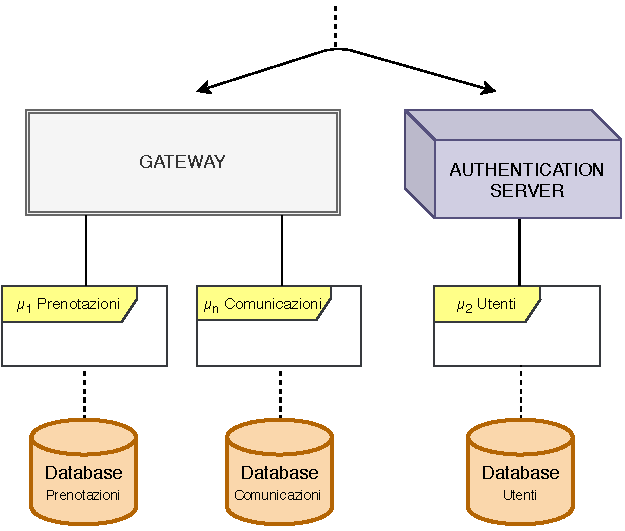
\includegraphics[width=0.70\textwidth]{images/02_7_ideal_architecture.pdf}
    \caption{Architettura Ideale del Sistema}
    \label{fig:idealarchitecture}
\end{figure}
Questa condizione risulta necessaria in un contesto di evoluzione del sistema. Oggi, tuttavia, essendo questa prima fase del refactoring non mirata alla ristrutturazione del database, questo tipo di architettura non è attuabile. La sua implementazione risulterà possibile solo in fase di completamento del refactoring.

%%%%%%%%%%%%%%%%%%%%%%%%%%%%%%%%%%%%%%%%%%%%%%%%%%%%%%%%%%%%%%%

% BIBLIOGRAFIA
\phantomsection
\addcontentsline{toc}{chapter}{\refname}
\nocite{*}
\printbibliography

\end{document}